\chapter{Introduction}\label{introduction}

This thesis presents an execution stack for neural networks using the
\emph{Kubernetes}\footnote{https://kubernetes.io} container
orchestration and a Java based microservice architecture, which is
exposed to users and other systems via RESTful web services and a web
frontend. The whole workflow including importing, training and
evaluating a neural network model, becomes possible by using this
service oriented approach (SOA). The presented stack runs on popular
cloud platforms, like \emph{Google Cloud Platform}\footnote{https://cloud.google.com/kubernetes-engine},
\emph{Amazon AWS}\footnote{https://aws.amazon.com/eks} and
\emph{Microsoft Azure}\footnote{https://azure.microsoft.com/services/container-service}.
Furthermore it is scalable and each component is extensible and
interchangeable. This work is influenced by N2Sky \cite{schikuta_2013},
a framework to exchange neural network specific knowledge and aims to
support \emph{ViNNSL}, the Vienna Neural Network Specification Language
\cite{kopica_2015} \cite{beran_2008}.

\paragraph{Objectives:}\label{objectives}

The first objective is to specify functional and non-functional
requirements for the neural network system. This is followed by the
characterisation of the API and the implemention of microservices that
later define the neural network composition as a collection of loosly
coupled services.

The next step is to setup a \emph{Kubernetes} cluster to create the
foundation of container orchestration.

Finally the microservices are deployed to containers and combined in a
cluster.

\paragraph{Non-Objectives:}\label{non-objectives}

The prototype does not fully implement the \emph{ViNNSL} in version 2.0,
as described in \cite{kopica_2015} and provides limited data in-/output.
Limitations are described in section TODO.

\section{Problem Statement}\label{problem-statement}

Getting started with machine learning and in particular with neural
networks is not a trivial task. It is a complex field with a high entry
barrier and requires most often programming skills and expertise in
neural network frameworks. In most cases a complex setup is needed to
train and evaluate networks, which is both a processor- and
memory-intense job. With cloud computing getting more and more
affordable and powerful, it makes sense to shift these tasks into the
cloud. There are already existing cloud platforms for machine learning,
but to my present research all of them do not fulfil at least one of the
following criteria:

\begin{itemize}
\tightlist
\item
  platform is open-source
\item
  no programming skills required to define and train a neural network
  model
\item
  can be deployed on-site and and in the cloud
\item
  components extensible and replaceable by developers
\item
  provides a RESTful interface
\end{itemize}

This thesis showcases an architecture, that tries to achieve all of
that.

\section{Motivation}\label{motivation}

Machine learning has become a highly discussed topic in information
technology in the past years and the trend is further increasing. It has
become an essential part of everyday life when using search engines or
speech recognition systems, like personal assistants. Self-learning
algorithms in applications learn from the input of their users and
decide which news an individual should read next, which song to listen
to or which social media post should appear first. Messages are being
analyzed and possible answers automatically predicted.

A recent Californian study shows that 6.5 million developers worldwide
are currently involved in projects that use artificial intelligence
techniques and another 5.8 million developers expect to implement these
in near future \cite{evans}.

Machine learning is not just a business area in the United States,
survey results of 264 companies in the DACH region show, that 56 of them
already use that kind of technology in production. In the near future
112 companies plan to do so or already have initial experiences (see
figure \ref{img.crisp_ml_verbreitung}). It is seen by a fifth of the
decision-makers as a core area to improve the competitiveness and
profitability of companies in future. \cite{crisp}

\begin{figure}
\centering
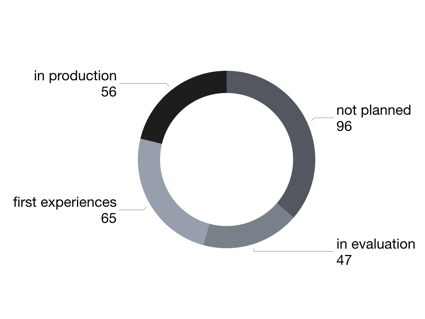
\includegraphics[width=10.00000cm]{images/crisp_ml_verbreitung}
\caption{Distribution of machine learning of 264 companies in the DACH
region \cite{crisp}\label{img.crisp_ml_verbreitung}}
\end{figure}

At the same time more and more companies shift their business logic from
a monolithic design to microservices. Each service is dedicated to a
single task that can be developed, deployed, replaced and scaled
independently. Test results have shown that not only this architecture
can help reduce infrastructure costs
\cite{villamizar2}\cite{villamizar}, but also reduces complexity of the
code base and enables applications to dynamically adjust computing
resources on demand \cite{villamizar}.

The presented project combines these techniques and demonstrates a
prototype that is open-source and is supported by common cloud
providers. Developers can integrate their own solutions into the
platform or exchange components ad libitum.

It also integrates with ViNNSL, a descriptive language that does not
require programming skills to define, train and evaluate neural
networks.

\section{Structure}\label{structure}

TODO

\chapter{State of the Art}\label{state-of-the-art}

\section{Containers}\label{containers}

\subsection{Docker Containers}\label{docker-containers}

Containers enable software developers to deploy applications that are
portable and consistent across different environments and providers
\cite{baier-kub} by running isolated on top of the operating system's
kernel \cite{bashari}. As an organisation, Docker\footnote{https://docker.com}
has seen an increase of popularity very quickly, mainly because of its
advantages, which are speed, portability, scalability, rapid delivery,
and density \cite{bashari}.

Building a Docker container is fast, because images do not include a
guest operating system. The container format itself is standardized,
which means that developers only have to ensure that their application
runs inside the container, which is then bundled into a single unit. The
unit can be deployed on any Linux system as well as on various cloud
environments and therefore easily be scaled. Not using a full operating
system makes containers use less resources than virtual machines, which
ensures higher workloads with greater density. \cite{joy2015}

\section{Microservices}\label{microservices}

The micoservice architecture pattern is a variant of a service-oriented
architecture (SOA). An often cited definition originates from Martin
Fowler and James Lewis:

\begin{quote}
In short, the microservice architectural style is an approach to
developing a single application as a suite of small services, each
running in its own process and communicating with lightweight
mechanisms, often an HTTP resource API. These services are built around
business capabilities and independently deployable by fully automated
deployment machinery. There is a bare minimum of centralized management
of these services, which may be written in different programming
languages and use different data storage technologies.
\cite{lewis2014microservices}
\end{quote}

Figure \ref{monolithic_vs_microservice} shows the architectural
difference between the monolithic and microservice architecture.
Monolithic applications bundle user interface, data access layer and
business logic together a single unit. In the microservice architecture
each task has its own service. The user interface puts information
together from multiple services.

\begin{figure}
\centering
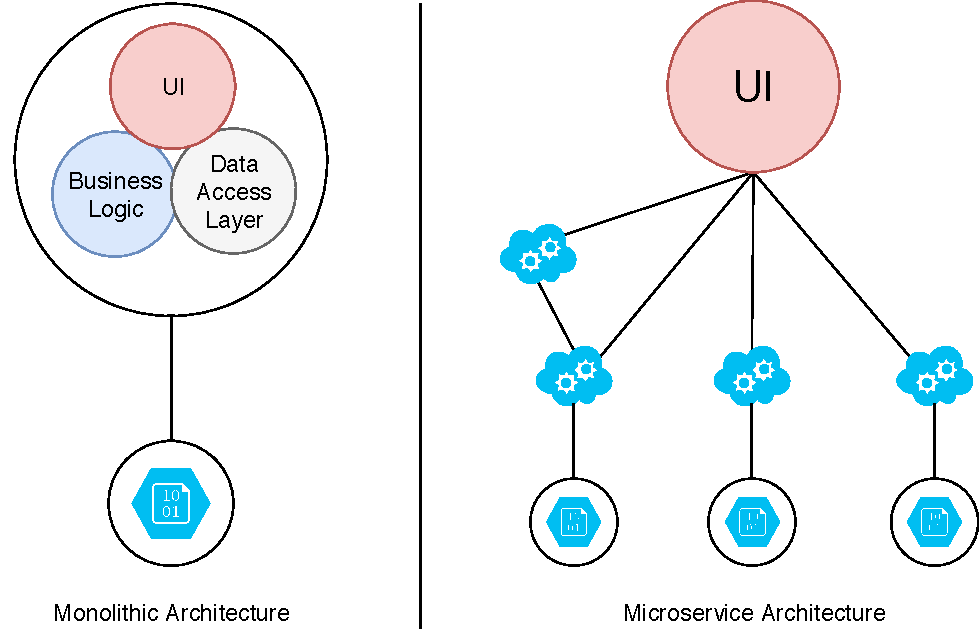
\includegraphics[width=15.00000cm]{images/monolithic_vs_microservice}
\caption{Monolithic Architecture vs.~Microservice Architecture
\label{monolithic_vs_microservice}}
\end{figure}

\section{Container Orchestration
Technologies}\label{container-orchestration-technologies}

\subsection{Kubernetes}\label{kubernetes}

Kubernetes is the third container-management system (after Borg and
Omega) developed by Google \cite{Burns:2016uq} for administering
applications, that are provided in containers, in a cluster of nodes.
Services that are responsible for controlling the cluster, are called
master components \cite{kub_intro}. Figure
\ref{kubernetes_core_architecture} shows the Kubernetes core
architecture, which includes the Master server, the nodes and the
interaction between the components.

\begin{figure}
\centering
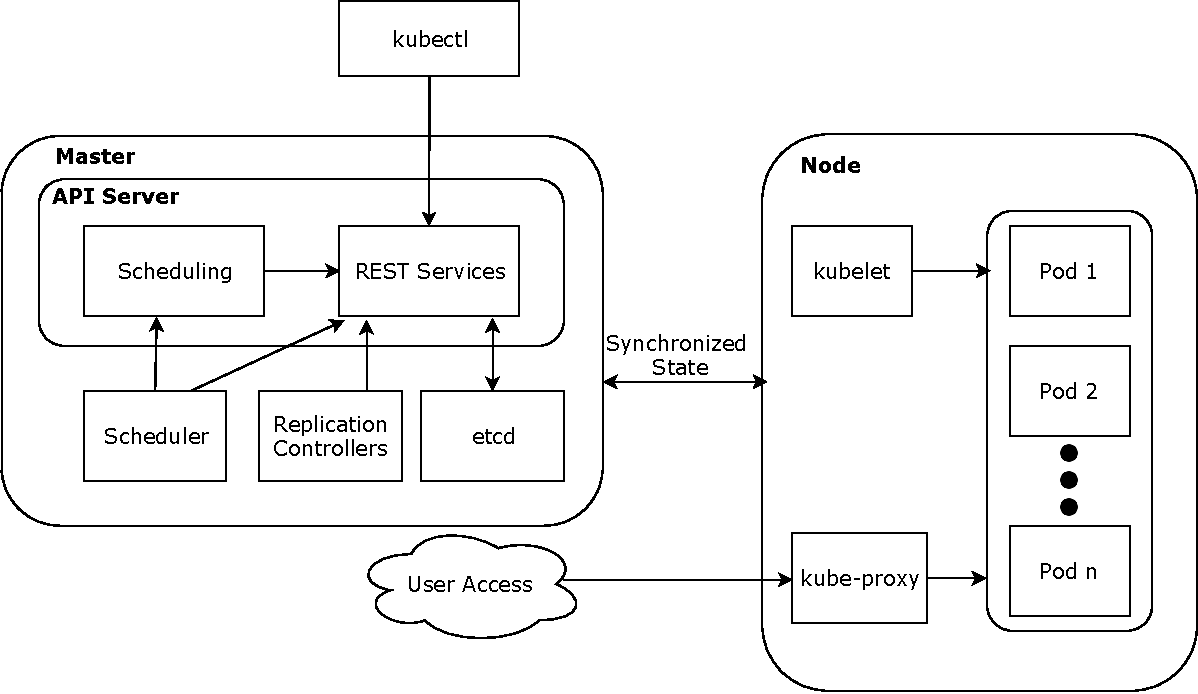
\includegraphics[width=15.00000cm]{images/kubernetes_core_architecture}
\caption{Kubernetes core
architecture\label{kubernetes_core_architecture}}
\end{figure}

\subsubsection{Master Components}\label{master-components}

The master consists of the core API server, that provides information
about the cluster and workload state and allows to define the desired
state \cite{baier-kub}. The master server also takes care of scheduling
and scaling workloads, cluster-wide networking and performs health
checks \cite{kub_intro}. Workloads are managed in form of so-called
pods, which are various containers that conclude the application stacks
\cite{baier-kub}.

\paragraph{etcd}\label{etcd}

etcd is a key-value store, accessible by a HTTP/JSON API, which can be
distributed across multiple nodes and is used by Kubernetes to store
configuration data, which needs to be accessible across nodes deployed
in the cluster. It is essential for service discovery and to describe
the state of the cluster, among other things. \cite{kub_intro}

etcd can also watch values for changes \cite{baier-kub}.

\paragraph{kube-apiserver}\label{kube-apiserver}

The API server acts as the main management point for the cluster and
provides a RESTful interface for users and other services to configure
workloads in the cluster. It is a bridge between other master components
and is responsible of maintaining health and spreading commands in the
cluster. \cite{kub_intro}

\paragraph{kube-scheduler}\label{kube-scheduler}

The scheduler keeps track of available and allocated resources on each
specific node in the cluster. It has an overview of the infrastructure
environment and needs to distribute workload to an acceptable node
without exceeding the available resources. Therefore each workload has
to declare its operating requirements. \cite{kub_intro}

\paragraph{kube-controller-manager}\label{kube-controller-manager}

The controller manager mainly operates different controllers that
constantly check the shared state of the cluster in \texttt{etcd} via
the apiserver \cite{kub_comp} and if the current state differs towards
the desired state it takes compensating measures \cite{kub_intro}.

For example the node controller's task is to react when nodes go offline
or down. The replication controller makes sure that the defined number
of desired pods is identical to the number of currently deployed pods in
the cluster and scales applications up or down accordingly. The
endpoints controller populates the endpoints to services \cite{kub_comp}

\paragraph{cloud-controller-manager}\label{cloud-controller-manager}

Kubernetes supports different cloud infrastructure providers. As each
cloud providers has different features, apis and capabilities, cloud
controller managers act as an abstraction to the generic internal
Kubernetes constructs. This has the advantage that the core Kubernetes
code is not dependent on cloud-provider-specific code. \cite{kub_comp}

\subsubsection{Node Components}\label{node-components}

Servers that accomplish workloads are called nodes. Each workload is
described as one or more containers that have to be deployed. Node
components run on every node in the cluster providing the Kubernetes
runtime environment \cite{kub_comp}, that establishes networking and
communicates with the master components. They also take care of
deploying the necessary containers on a node and keep them running
\cite{kub_intro}. Kubernetes requires a dedicated subnet for each node
server and a supported container runtime \cite{kub_comp}.

\paragraph{kubelet}\label{kubelet}

The kubelet is the primary agent running on each node in the cluster,
responsible for running pods \cite{kub_comp}. It communicates with the
API server to receive commands invoked by the scheduler. Interaction
takes place with the etcd store to read and update configuration and
state of the pod.

Pods are specified by the \emph{PodSpec}, which defines the workload and
parameters on how to run the containers \cite{kub_intro}. The kubelet
process is responsible that the containers described in the
specification are running and healthy \cite{kub_comp}.

\paragraph{kube-proxy}\label{kube-proxy}

The proxy service is in charge of forwarding requests of defined
services to the correct containers. On a basic level, load balancing is
also done by the proxy. \cite{baier-kub}

\paragraph{Container Runtime}\label{container-runtime}

The container runtime is an implementation running containers. Currently
Docker, rkt, runc and OpenContainer runtimes are supported.
\cite{kub_comp}

\paragraph{Pods}\label{pods}

A pod is the smallest deployable unit in a cluster consisting of a group
of one or more containers, which share network and storage.
\cite{kub-pod}

\subsubsection{Addons}\label{addons}

\paragraph{Cluster DNS}\label{cluster-dns}

Cluster DNS server keeps track of running services in the cluster and
updates DNS records accordingly. This allows an easy way of service
discovery. Containers include this DNS server in their DNS lookups
automatically -- that way a service can resolve another service by its
name. \cite{baier-kub}

\paragraph{Dashboard}\label{dashboard}

The dashboard is a web-based user interface that allows to manage
Kubernetes clusters and applications running in the cluster
\cite{kub_comp}. It also provides access to log messages in each pod.

\subsection{Docker Swarm}\label{docker-swarm}

https://github.com/GuillaumeRochat/container-orchestration-comparison

\section{Machine Learning}\label{machine-learning}

\emph{Machine learning---the process by which computers can get better
at performing tasks through exposure to data, rather than through
explicit programming---requires massive computational power, the kind
usually found in clusters of energy-guzzling, cloud-based computer
servers outfitted with specialized processors. But an emerging trend
promises to bring the power of machine learning to mobile devices that
may lack or have only intermittent online connectivity. This will give
rise to machines that sense, perceive, learn from, and respond to their
environment and their users, enabling the emergence of new product
categories, reshaping how businesses engage with customers, and
transforming how work gets done across
industries.(https://www2.deloitte.com/insights/us/en/focus/signals-for-strategists/machine-learning-mobile-applications.html)}
TODO CITATION

\subsection{Classification}\label{classification}

\subsection{Neural Networks}\label{neural-networks}

\subsubsection{Tensorflow}\label{tensorflow}

\subsubsection{DL4J}\label{dl4j}

\chapter{Requirements}\label{requirements}

\section{Functional Requirements}\label{functional-requirements}

TODO

\begin{itemize}
\tightlist
\item
  NN in Cloud Rechnen
\item
  Verwendung der verständlichen Beschreibungssprache ViNNSl
\item
  all Devices, from everywhere
\item
  berechnetes Netzwerk kann in eig App verwendet werden / oder als
  Webservice exposed
\end{itemize}

\subsection{User Interface}\label{user-interface}

\subsubsection{Mockup}\label{mockup}

TODO

Figure \ref{vinnsl-ui-mockup} shows a sketch of the user interface.

\begin{figure}
\centering
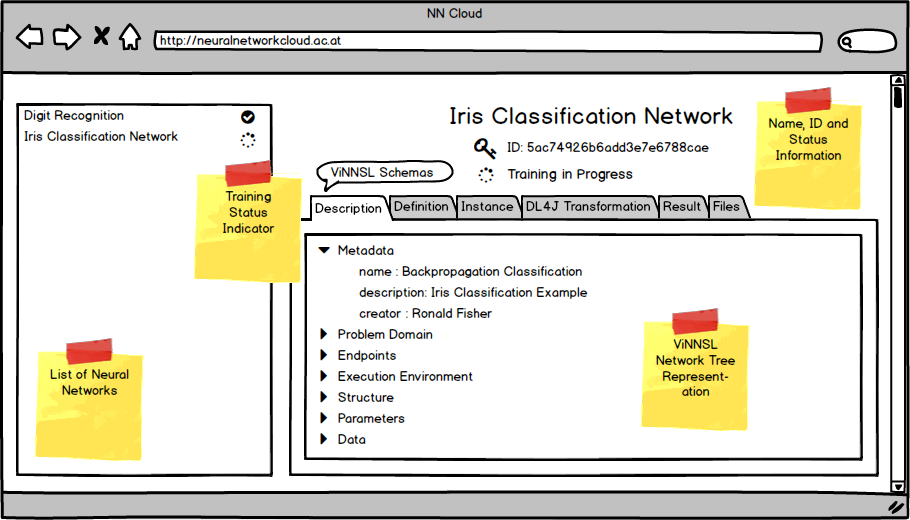
\includegraphics[width=17.00000cm]{./images/vinnsl-ui-mockup}
\caption{Mockup: User Interface of Frontend
Service\label{vinnsl-ui-mockup}}
\end{figure}

\section{Non-Functional Requirements}\label{non-functional-requirements}

\subsection{Quality}\label{quality}

\subsection{Technical}\label{technical}

\subsection{Software}\label{software}

\subsection{Hardware}\label{hardware}

\subsection{Documentation}\label{documentation}

\subsection{Developer Environment}\label{developer-environment}

\chapter{Specification}\label{specification}

\section{Use Case}\label{use-case}

Figure \ref{img.use_case_nn} shows the UML use case diagram.

\subsection{Use Case Descriptions}\label{use-case-descriptions}

TODO (hinzufügen: dev: kann trainiertes netz in eigener app verwenden
,data scientist: trainiertes netzwerk exportieren und developer
überreichen)

\begin{figure}
\centering
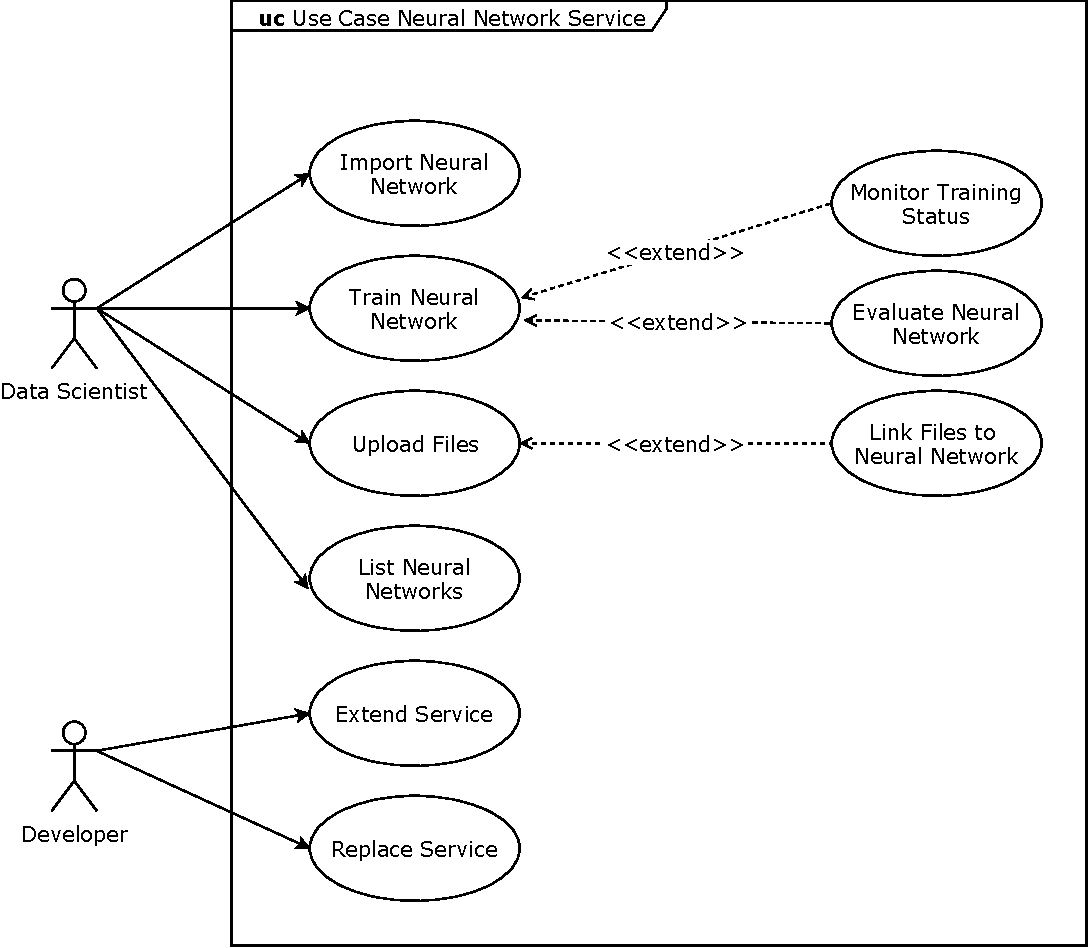
\includegraphics[width=15.00000cm]{images/use_case_nn}
\caption{UML Use Case Diagram \label{img.use_case_nn}}
\end{figure}

\section{Sequence Diagram}\label{sequence-diagram}

\subsection{Sequence of Training}\label{sequence-of-training}

TODO

Figure \ref{img.training_sequence} shows the sequence diagram.

\begin{figure}
\centering
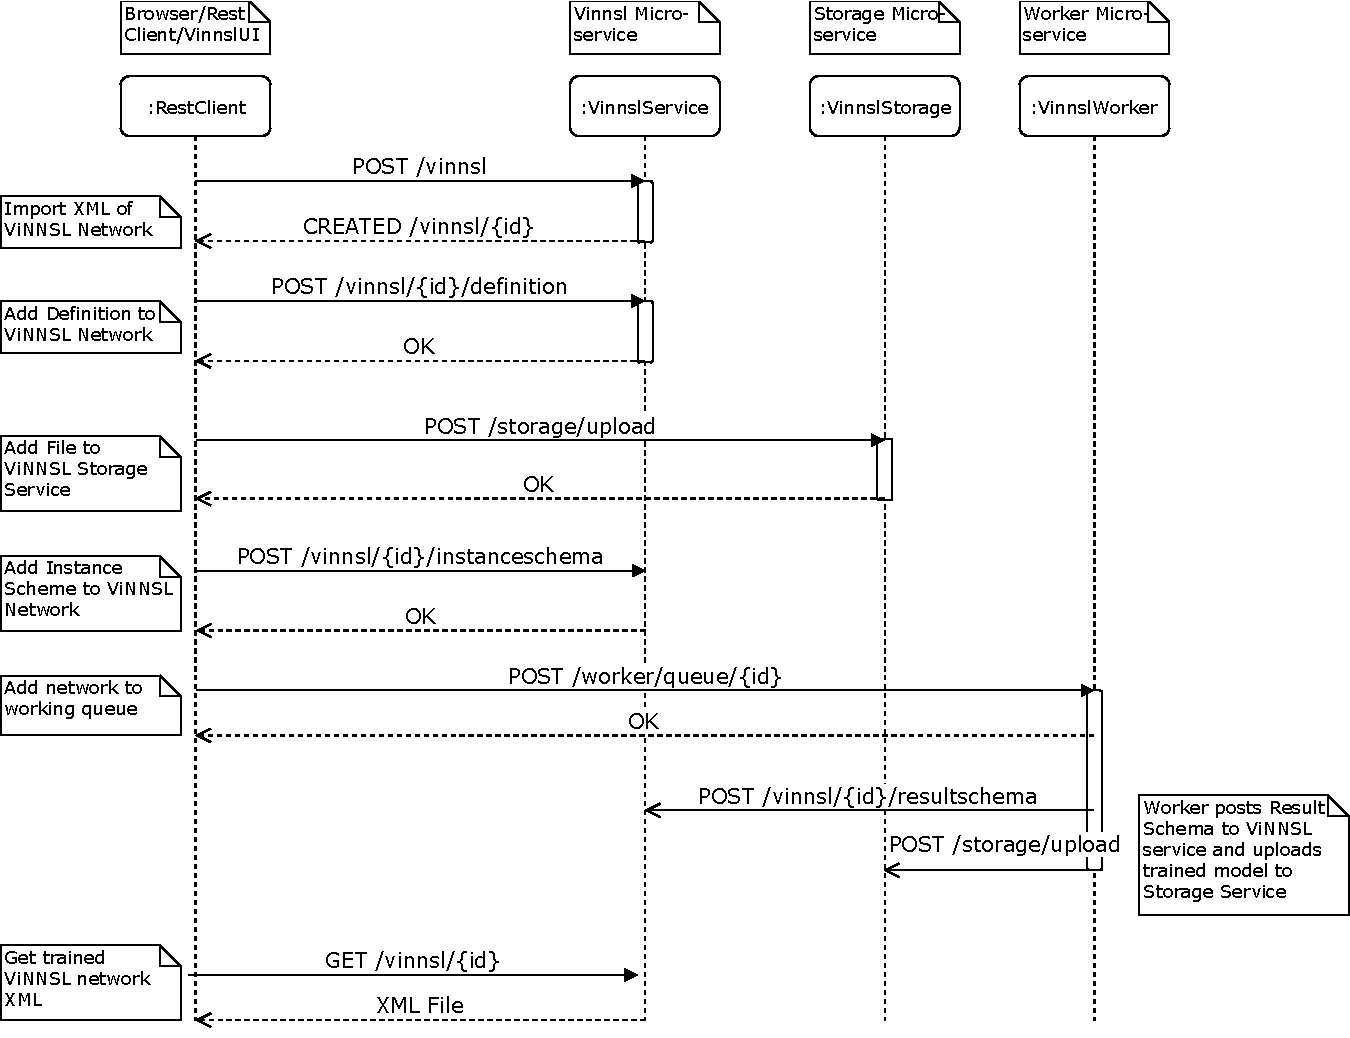
\includegraphics[width=15.00000cm]{images/training_sequence}
\caption{Training Sequence Diagram \label{img.training_sequence}}
\end{figure}

\section{Data Model Design}\label{data-model-design}

TODO

Figure \ref{img.db_schema} shows the data schema.

\begin{figure}
\centering
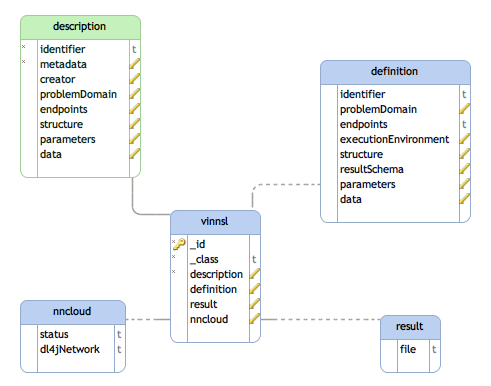
\includegraphics[width=15.00000cm]{images/db_schema}
\caption{NoSQL Data Model \label{img.db_schema}}
\end{figure}

\section{Overview Microservices}\label{overview-microservices}

The neural network cloud execution stack consists of four main services
that expose a RESTful API to users and two supporting services in charge
of persisting data. Figure \ref{img.overview_main_services} shows an
overview of these services.

\subsection{Vinnsl Service
(vinnsl-service)}\label{vinnsl-service-vinnsl-service}

The \texttt{vinnsl-service} is responsible for handling the import,
management and manipulation of neural network objects and it's status.
It maps the CRUD\footnote{Create, Read, Update, Delete} operations to
HTTP methods. A new neural network is created by sending a \texttt{POST}
request to the \texttt{/vinnsl} endpoint containing a ViNNSL Definition
XML as body. Sending a \texttt{GET} request to the \texttt{/vinnsl}
route returns a JSON containing all ViNNSL neural network objects.

The \texttt{vinnsl-service} depends on the \texttt{vinnsl-db} service,
which runs a MongoDB database to store the objects.

\subsection{Worker Service
(vinnsl-nn-worker)}\label{worker-service-vinnsl-nn-worker}

The \texttt{vinnsl-nn-worker} implements a queue management for neural
network training and transforms ViNNSL neural network models into DL4J
models. It provides a wrapper of the DL4J platform, that handles the
training or evaluation of the network.

\subsection{Storage Service
(vinnsl-storage-service)}\label{storage-service-vinnsl-storage-service}

Binary files, like trained network models, images or csv files are
essential in the pocess of creating and training neural networks. File
management is handled by the \texttt{vinnsl-storage-service}.

\subsection{Frontend UI (vinnsl-nn-ui)}\label{frontend-ui-vinnsl-nn-ui}

The Frontend UI is a web application that gives a brief overview of all
neural network models, their training status and linked files.

\section{User Interface Design}\label{user-interface-design}

Auf Grundlage des ersten Sketches, wurde ein erstes Designmodell
entwickelt.

Figure \ref{vinnsl-ui-design} shows the user interface design for the
frontend web service.

\begin{figure}
\centering
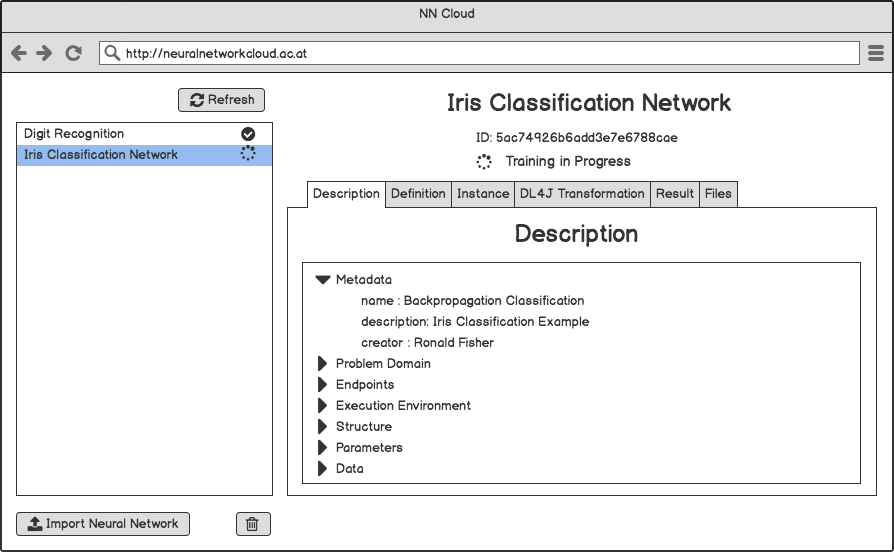
\includegraphics[width=17.00000cm]{images/vinnsl-ui-design}
\caption{User Interface Design for vinnsl-nn-ui\label{vinnsl-ui-design}}
\end{figure}

\section{Service Discovery and Load
Balancing}\label{service-discovery-and-load-balancing}

\begin{figure}
\centering
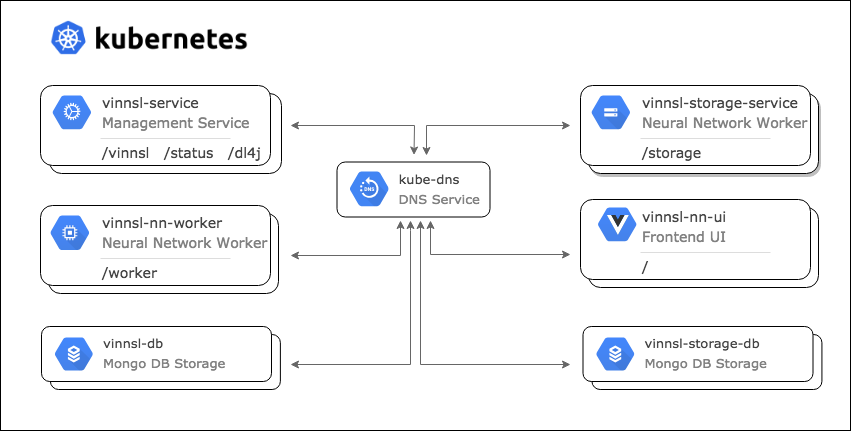
\includegraphics[width=15.00000cm]{images/overview_main_services}
\caption{Service Discovery with kube-dns}
\end{figure}

\section{Neural Network Objects}\label{neural-network-objects}

\subsection{State of Neural Network
Objects}\label{state-of-neural-network-objects}

\begin{figure}
\centering
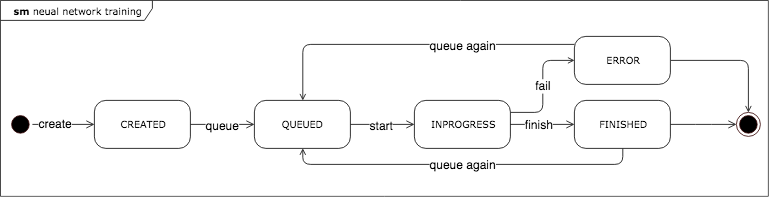
\includegraphics[width=15.00000cm]{images/nn-states}
\caption{State Machine of a Neural Network}
\end{figure}

\section{Class Diagram}\label{class-diagram}

\subsection{vinnsl-service}\label{vinnsl-service}

\begin{figure}
\centering
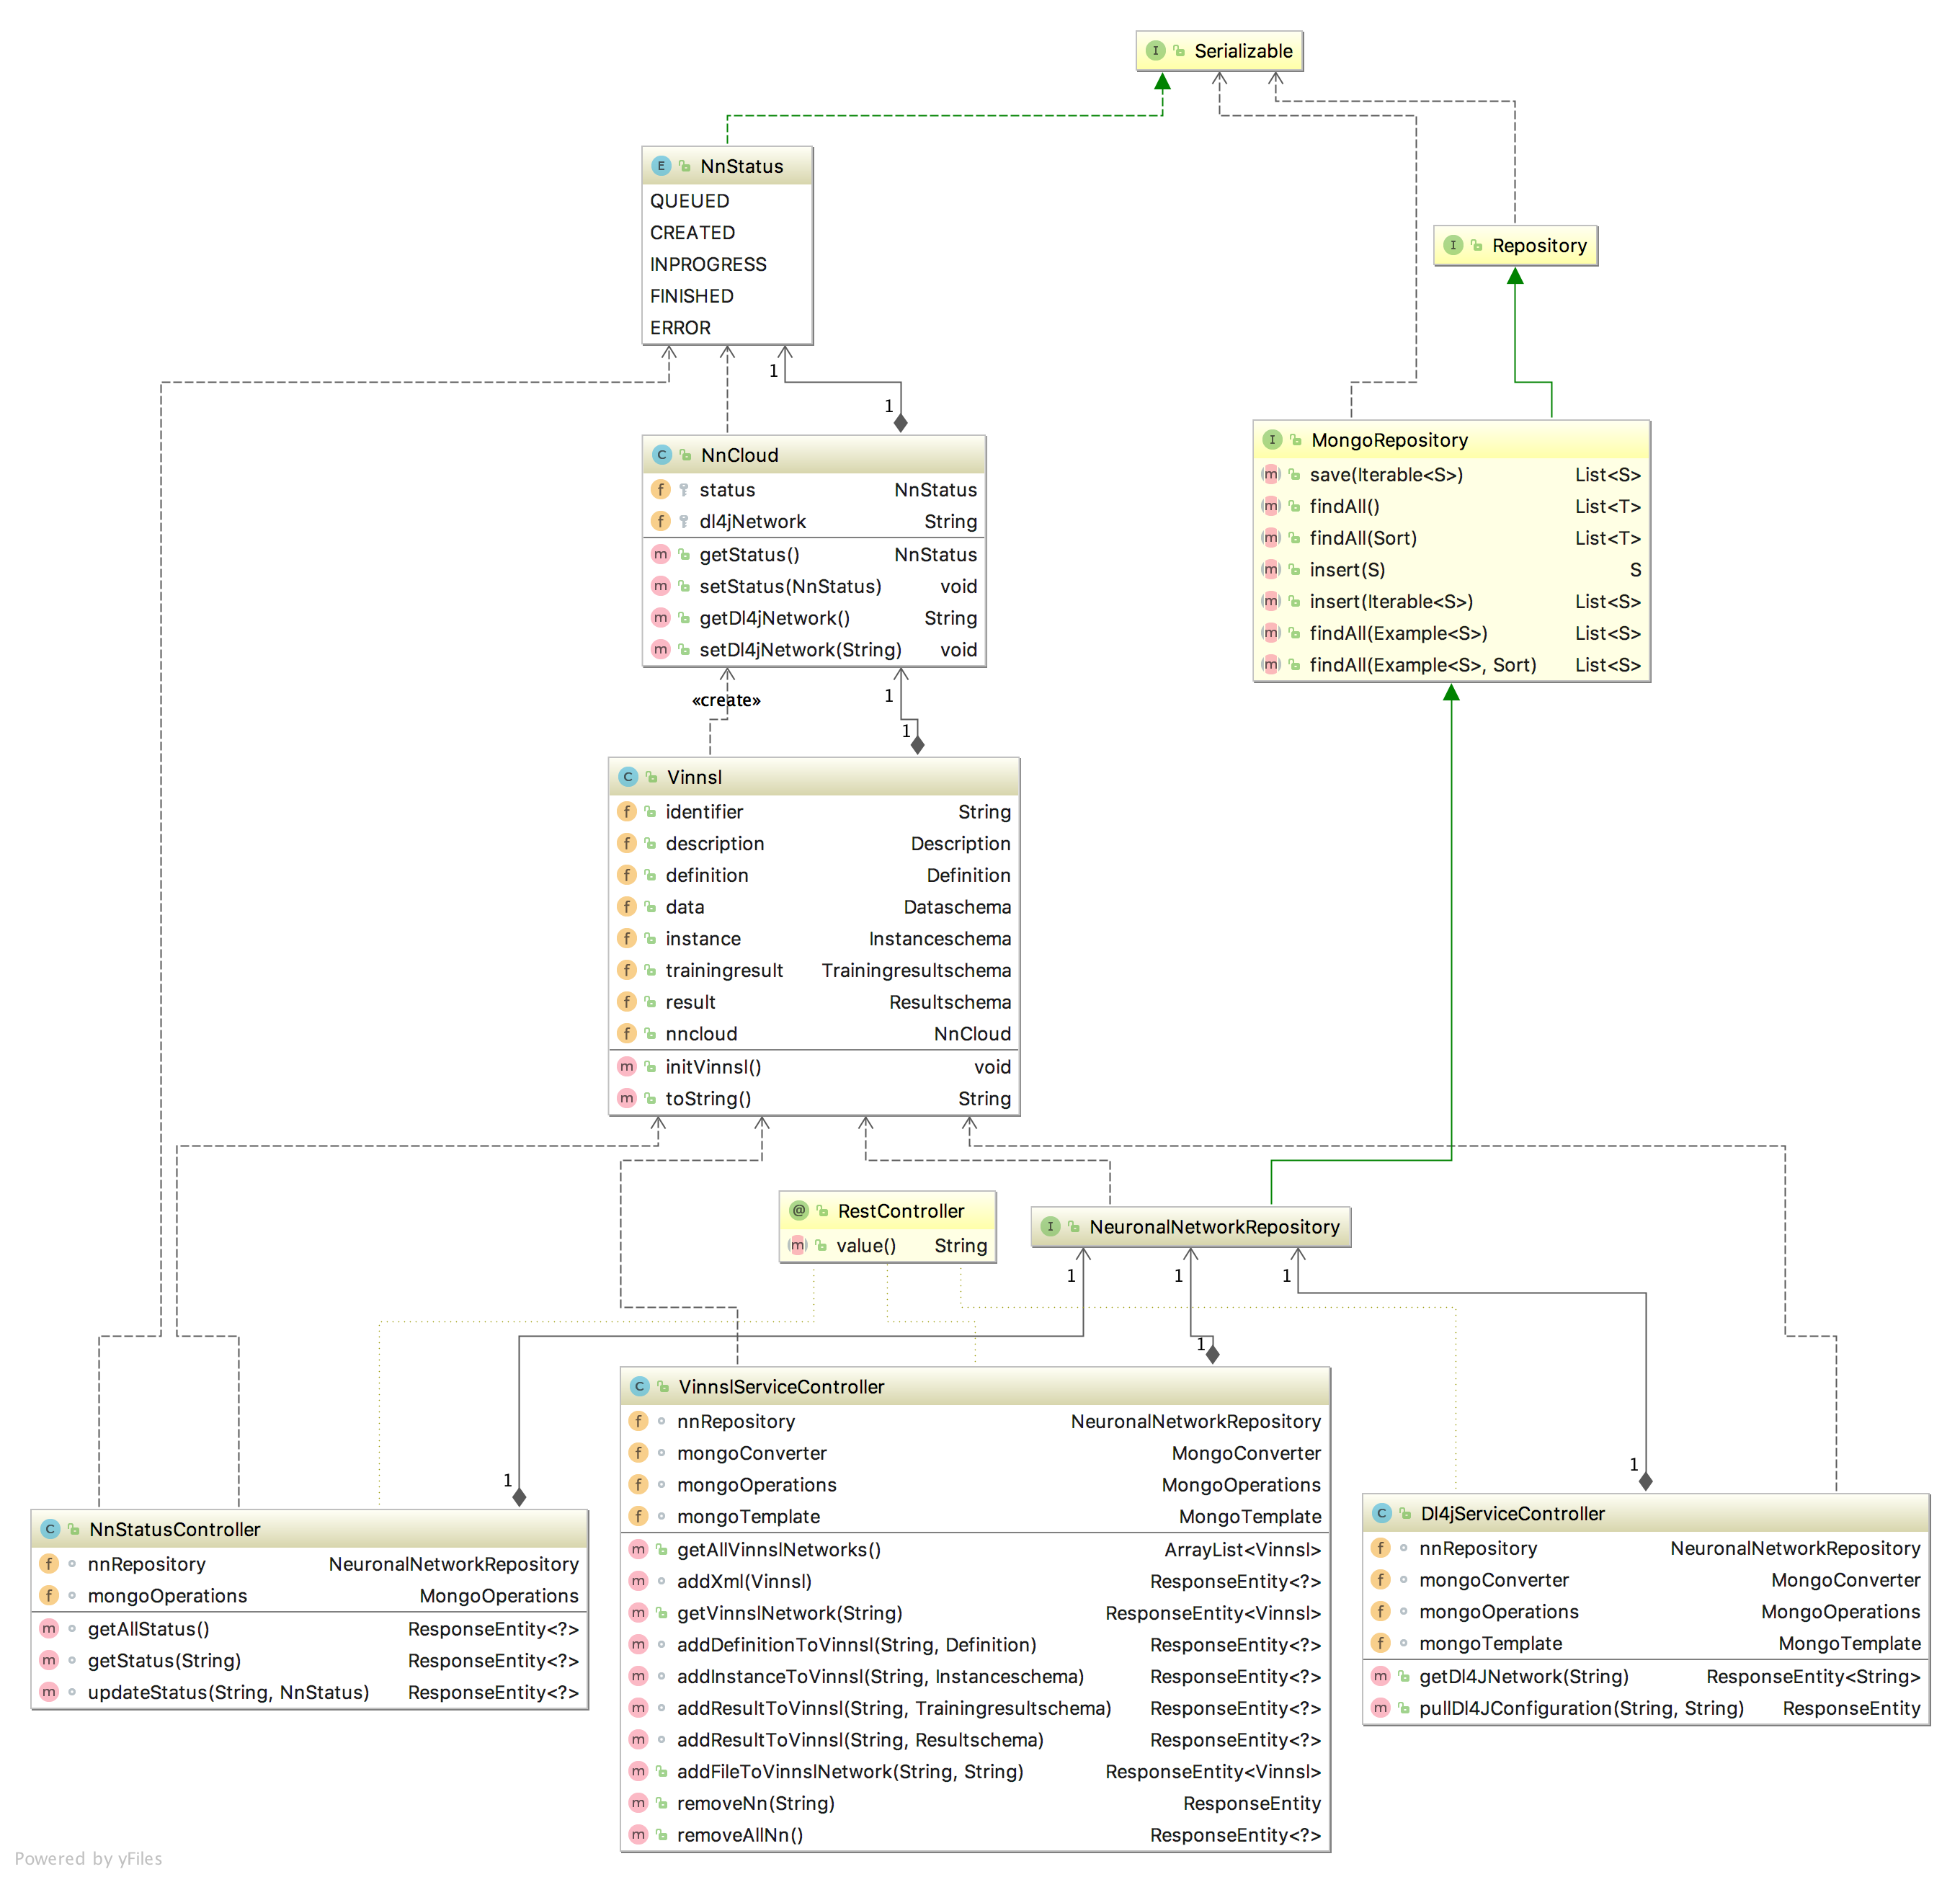
\includegraphics[width=17.00000cm]{images/uml-class-diagram-vinnsl-service}
\caption{Class Diagram of vinnsl-service}
\end{figure}

\subsection{vinnsl-storage-service}\label{vinnsl-storage-service}

\begin{figure}
\centering
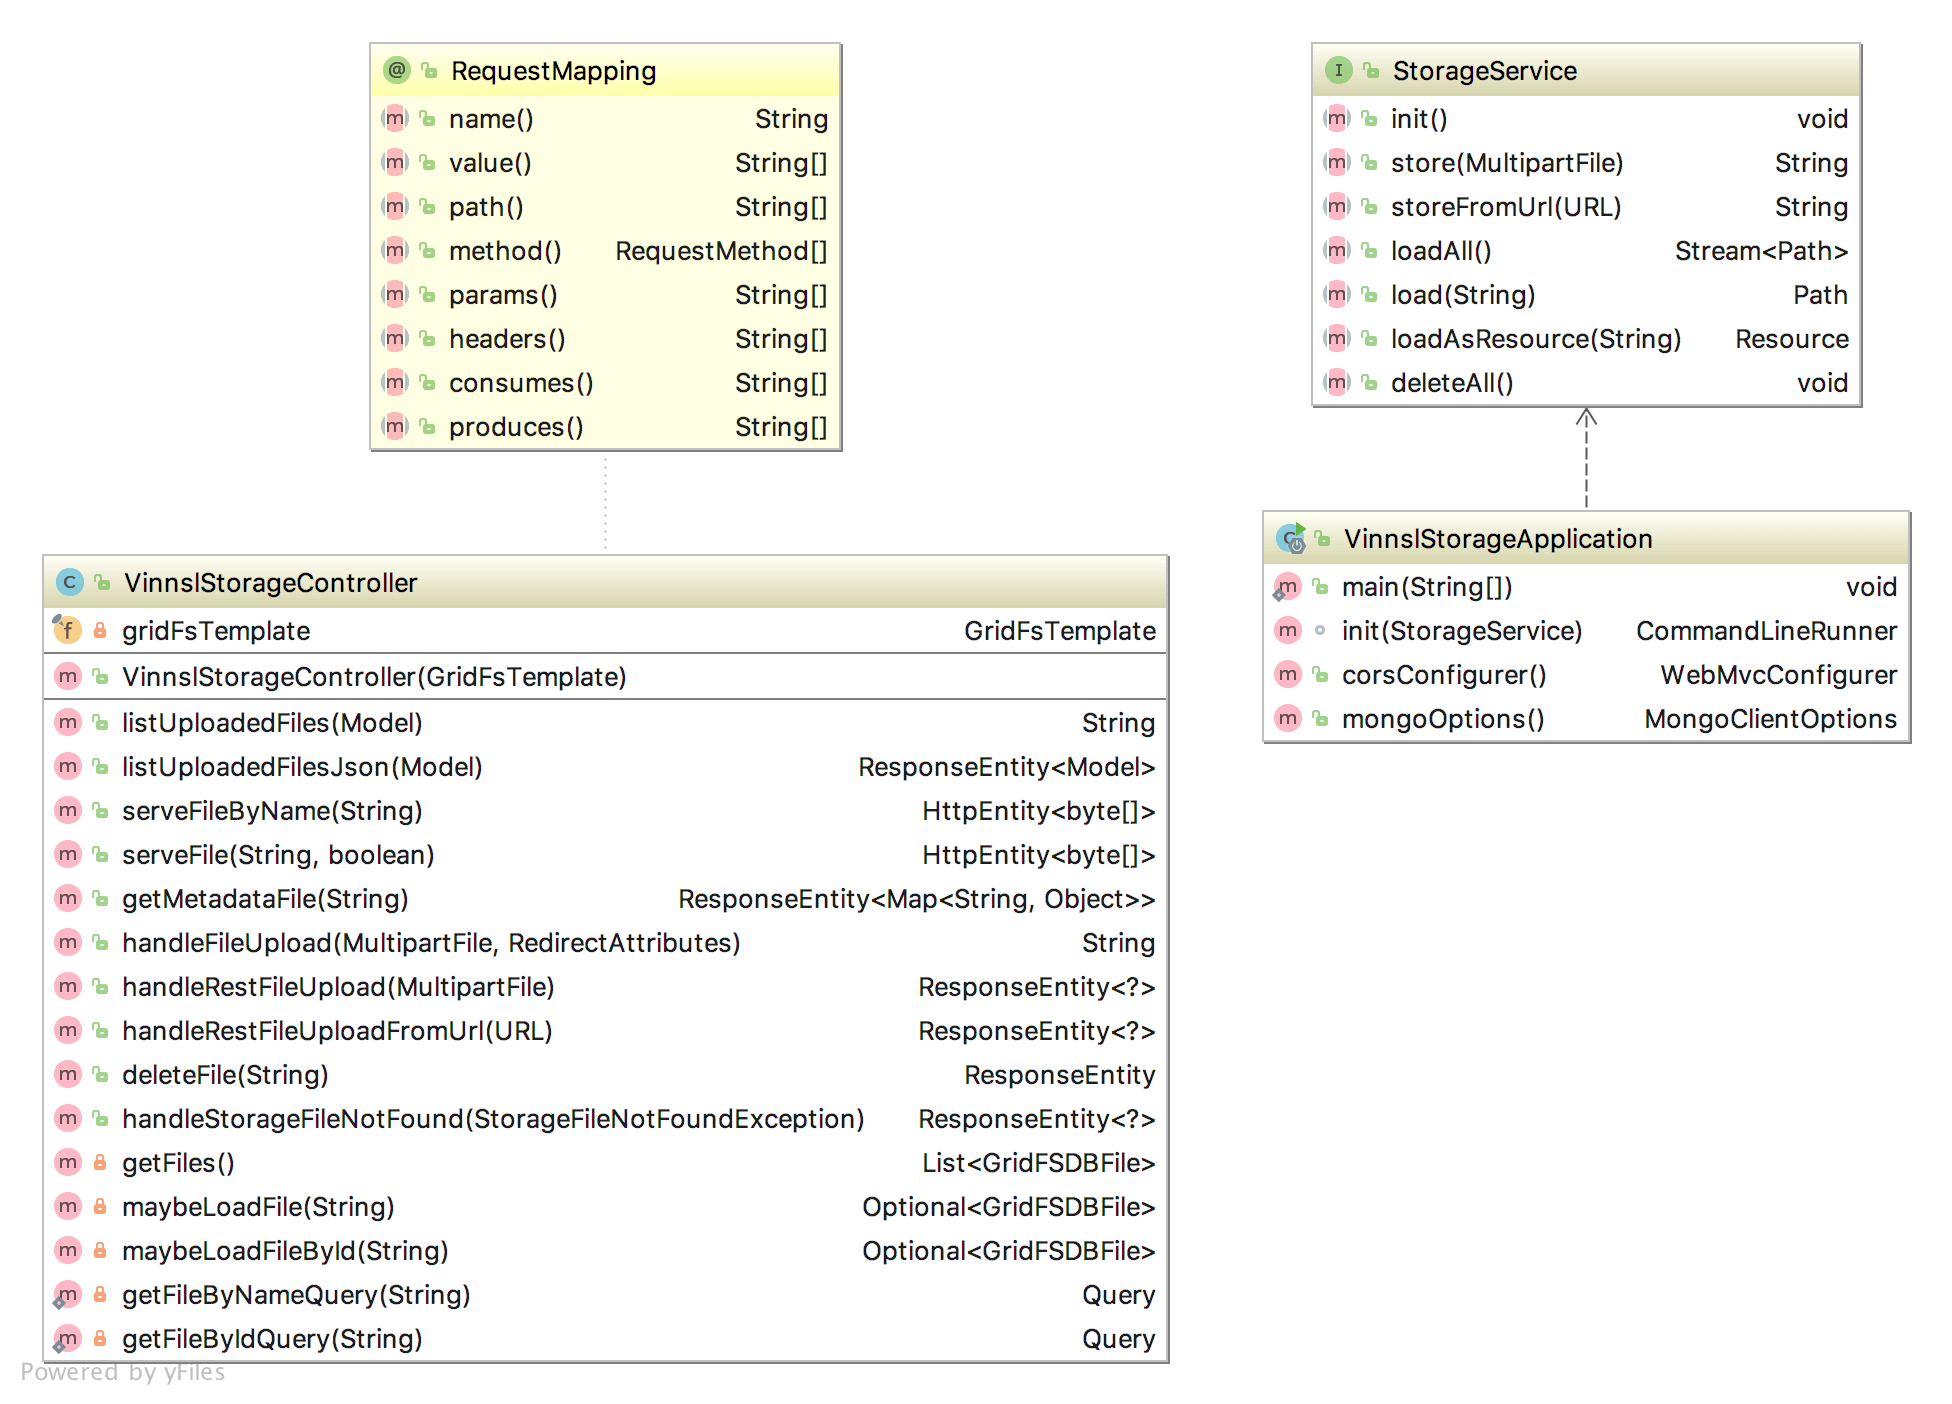
\includegraphics[width=15.00000cm]{images/uml-class-diagram-vinnsl-storage-service}
\caption{Class Diagram of vinnsl-storage-service}
\end{figure}

\subsection{vinnsl-worker-service}\label{vinnsl-worker-service}

\begin{figure}
\centering
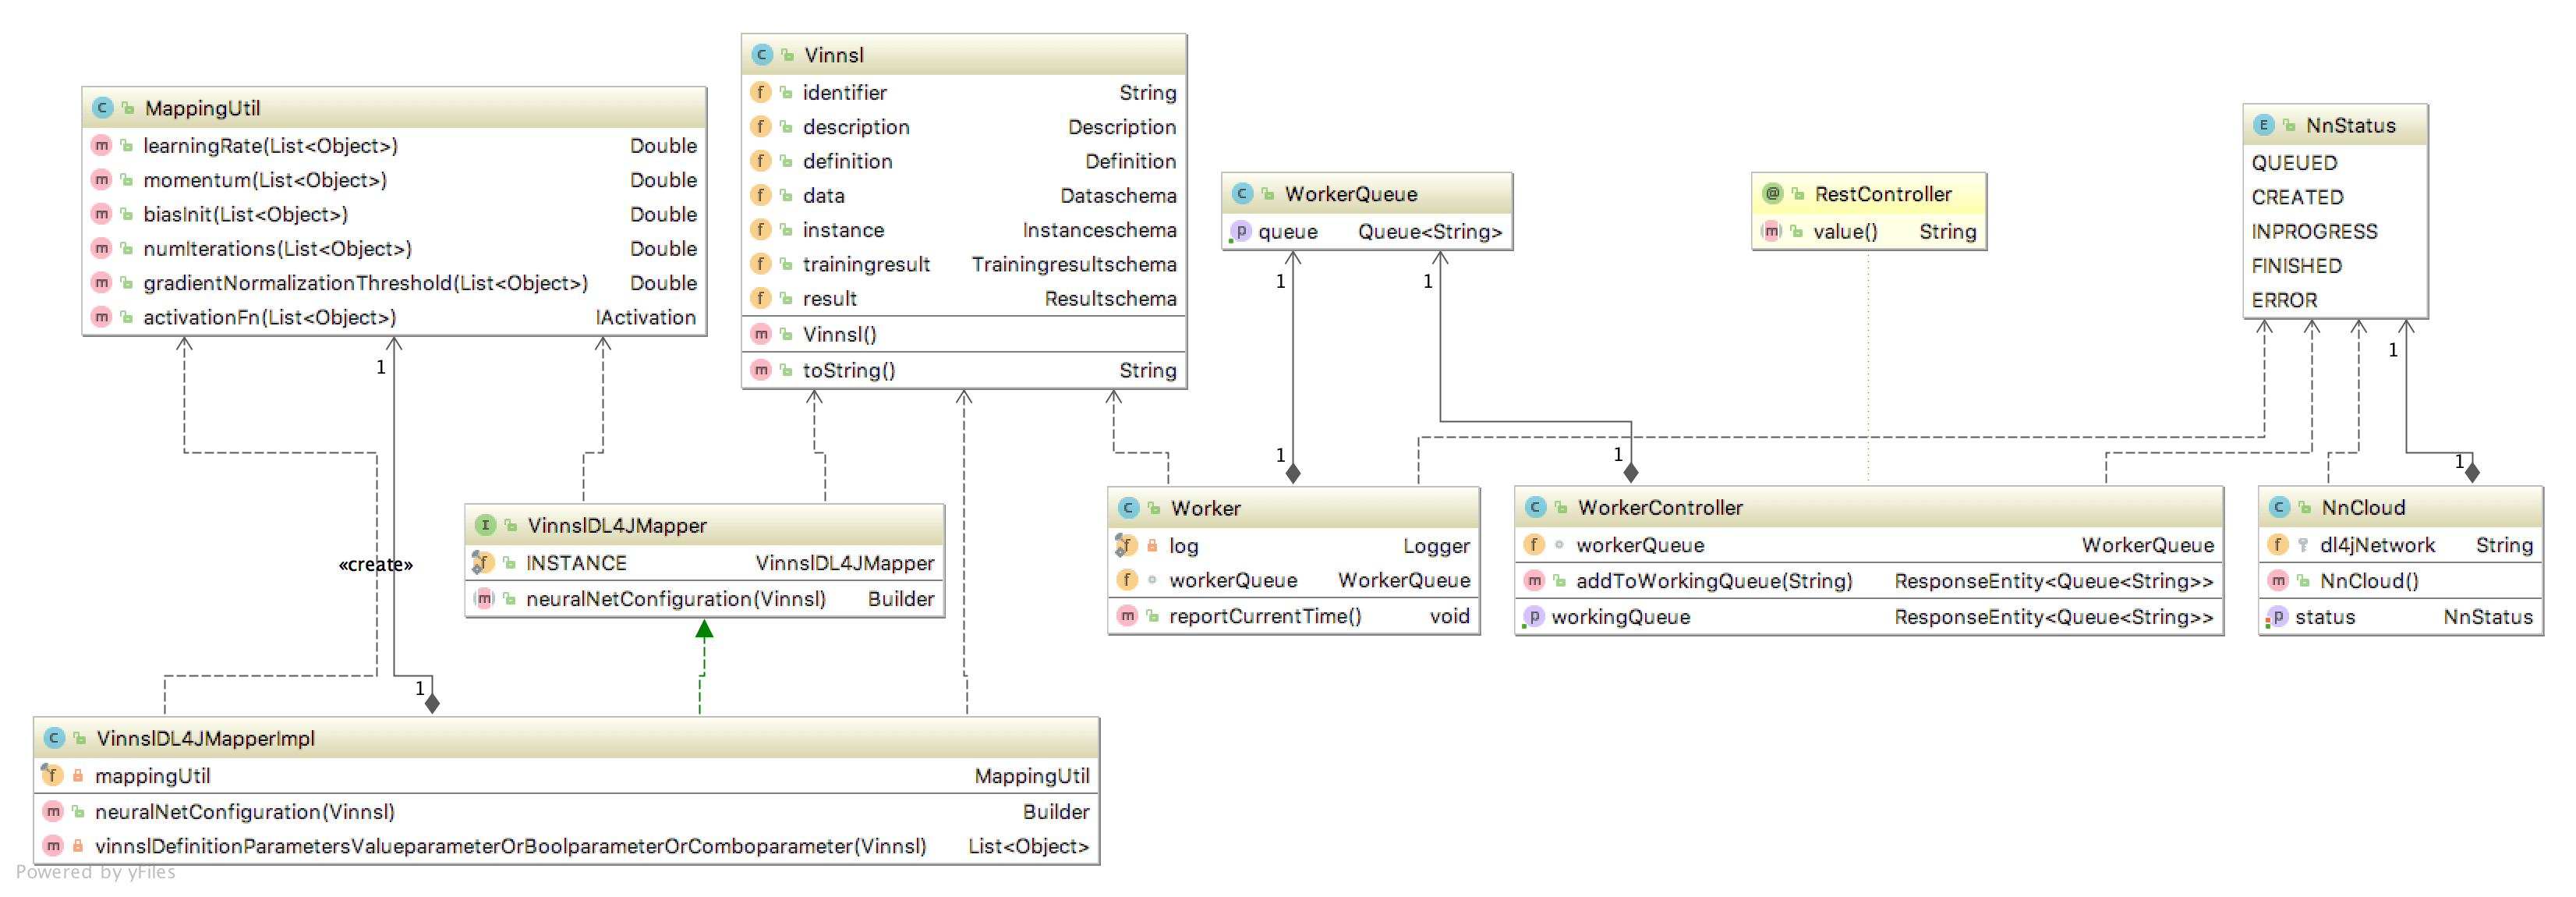
\includegraphics[width=17.00000cm]{images/uml-class-diagram-vinnsl-worker-service}
\caption{Class Diagram of vinnsl-worker-service}
\end{figure}

\chapter{REST API Documentation}\label{rest-api-documentation}

\paragraph{Base URL}\label{base-url}

\begin{verbatim}
http[s]://<clusterip>
\end{verbatim}

\section{vinnsl-service}\label{vinnsl-service-1}

\subsection{Import a new ViNNSL XML
Defintion}\label{import-a-new-vinnsl-xml-defintion}

\begin{verbatim}
POST /vinnsl
\end{verbatim}

\subsubsection{Parameters}\label{parameters}

\begin{longtable}[]{@{}llll@{}}
\toprule
Type & Name & Description & Schema\tabularnewline
\midrule
\endhead
\textbf{Body} & \textbf{vinnsl} \emph{required} & vinnsl &
Vinnsl\tabularnewline
\bottomrule
\end{longtable}

\subsubsection{Responses}\label{responses}

\begin{longtable}[]{@{}lll@{}}
\toprule
HTTP Code & Description & Schema\tabularnewline
\midrule
\endhead
\textbf{201} & Created & No Content\tabularnewline
\textbf{500} & Server Error & Error\tabularnewline
\bottomrule
\end{longtable}

\subsubsection{Consumes}\label{consumes}

\begin{itemize}
\tightlist
\item
  \texttt{application/xml}
\end{itemize}

\subsubsection{Produces}\label{produces}

\begin{itemize}
\tightlist
\item
  \texttt{*/*}
\end{itemize}

\subsubsection{Tags}\label{tags}

\begin{itemize}
\tightlist
\item
  vinnsl-service-controller
\end{itemize}

\subsubsection{Example HTTP request}\label{example-http-request}

\paragraph{Header}\label{header}

\begin{verbatim}
Content-Type: application/xml
\end{verbatim}

\paragraph{Body}\label{body}

\begin{verbatim}
<vinnsl>
  <description>
    <identifier><!-- will be generated --></identifier>
    <metadata>
      <paradigm>classification</paradigm>
      <name>Backpropagation Classification</name>
      <description>Iris Classification Example</description>
      <version>
        <major>1</major>
        <minor>0</minor>
      </version>
    </metadata>
    <creator>
      <name>Ronald Fisher</name>
      <contact>ronald.fisher@institution.com</contact>
    </creator>
    <problemDomain>
      <propagationType type="feedforward">
        <learningType>supervised</learningType>
      </propagationType>
      <applicationField>Classification</applicationField>
      <networkType>Backpropagation</networkType>
      <problemType>Classifiers</problemType>
    </problemDomain>
    <endpoints>
      <train>true</train>
      <retrain>true</retrain>
      <evaluate>true</evaluate>
    </endpoints>
    <structure>
       <input>
        <ID>Input1</ID>
        <size>
            <min>4</min>
            <max>4</max>
        </size>
       </input>
       <hidden>
        <ID>Hidden1</ID>
        <size>
            <min>3</min>
            <max>3</max>
        </size>
       </hidden>
       <hidden>
        <ID>Hidden2</ID>
        <size>
            <min>3</min>
            <max>3</max>
        </size>
       </hidden>
       <output>
        <ID>Output1</ID>
        <size>
            <min>3</min>
            <max>3</max>
        </size>
       </output>
     </structure>
     <parameters/>
     <data>
        <description>iris txt file with 3 classifications, 4 input vars</description>
        <tabledescription>no input as table possible</tabledescription>
        <filedescription>CSV file</filedescription>
     </data>
  </description>
</vinnsl>
\end{verbatim}

\subsubsection{Example HTTP response}\label{example-http-response}

Statuscode: \texttt{201} CREATED

\paragraph{Header}\label{header-1}

\begin{verbatim}
Location: https://<baseURL>/vinnsl/5ade36bbd601800001206798
\end{verbatim}

\subsection{List all Neural Networks}\label{list-all-neural-networks}

\begin{verbatim}
GET /vinnsl
\end{verbatim}

\subsubsection{Responses}\label{responses-1}

\begin{longtable}[]{@{}lll@{}}
\toprule
HTTP Code & Description & Schema\tabularnewline
\midrule
\endhead
\textbf{200} & OK & \textless{} Vinnsl \textgreater{}
array\tabularnewline
\textbf{404} & Not Found & No Content\tabularnewline
\textbf{500} & Server Error & Error\tabularnewline
\bottomrule
\end{longtable}

\subsubsection{Produces}\label{produces-1}

\begin{itemize}
\tightlist
\item
  \texttt{application/json}
\end{itemize}

\subsubsection{Tags}\label{tags-1}

\begin{itemize}
\tightlist
\item
  vinnsl-service-controller
\end{itemize}

\subsubsection{Example HTTP Response}\label{example-http-response-1}

\begin{verbatim}
[
    {
        "identifier": "5ab91658e8cc45946600ea11",
        "description": {},
        "definition": {},
        "data": {},
        "instance": {},
        "trainingresult": {},
        "result": {},
        "nncloud": {
            "status": "CREATED",
            "dl4jNetwork": "{}
        }
    },
    ...
]
\end{verbatim}

\subsection{Delete all Neural
Networks}\label{delete-all-neural-networks}

\begin{verbatim}
DELETE /vinnsl/deleteall
\end{verbatim}

\subsubsection{Responses}\label{responses-2}

\begin{longtable}[]{@{}lll@{}}
\toprule
HTTP Code & Description & Schema\tabularnewline
\midrule
\endhead
\textbf{200} & OK & object\tabularnewline
\textbf{204} & No Content & No Content\tabularnewline
\textbf{500} & Server Error & Error\tabularnewline
\bottomrule
\end{longtable}

\subsubsection{Produces}\label{produces-2}

\begin{itemize}
\tightlist
\item
  \texttt{application/json}
\end{itemize}

\subsubsection{Tags}\label{tags-2}

\begin{itemize}
\tightlist
\item
  vinnsl-service-controller
\end{itemize}

\subsection{Get Neural Network Object}\label{get-neural-network-object}

\begin{verbatim}
GET /vinnsl/{id}
\end{verbatim}

\subsubsection{Parameters}\label{parameters-1}

\begin{longtable}[]{@{}llll@{}}
\toprule
Type & Name & Description & Schema\tabularnewline
\midrule
\endhead
\textbf{Path} & \textbf{id} \emph{required} & id & string\tabularnewline
\bottomrule
\end{longtable}

\subsubsection{Responses}\label{responses-3}

\begin{longtable}[]{@{}lll@{}}
\toprule
HTTP Code & Description & Schema\tabularnewline
\midrule
\endhead
\textbf{200} & OK & Vinnsl\tabularnewline
\textbf{404} & Not Found & No Content\tabularnewline
\bottomrule
\end{longtable}

\subsubsection{Produces}\label{produces-3}

\begin{itemize}
\tightlist
\item
  \texttt{application/xml}
\item
  \texttt{application/json}
\end{itemize}

\subsubsection{Tags}\label{tags-3}

\begin{itemize}
\tightlist
\item
  vinnsl-service-controller
\end{itemize}

\subsubsection{Example HTTP response}\label{example-http-response-2}

\begin{verbatim}
<?xml version="1.0" encoding="UTF-8" standalone="yes"?>
<vinnsl>
    <identifier>5ab91658e8cc45946600ea11</identifier>
    <description>
        <identifier></identifier>
        <metadata>
            <paradigm>classification</paradigm>
            <name>Backpropagation Classification</name>
            <description>Face Recognition Example</description>
            <version>
                <major>1</major>
                <minor>5</minor>
            </version>
        </metadata>
        <creator>
            <name>Autor 1</name>
            <contact>author1@institution.com</contact>
        </creator>
        <problemDomain>
            <propagationType type="feedforward">
                <learningType>supervised</learningType>
            </propagationType>
            <applicationField>EMS</applicationField>
            <applicationField>Operations</applicationField>
            <applicationField>FaceRecoginition</applicationField>
            <networkType>Backpropagation</networkType>
            <problemType>Classifiers</problemType>
        </problemDomain>
        <endpoints>
            <train>true</train>
            <retrain>true</retrain>
            <evaluate>true</evaluate>
        </endpoints>
        <structure>
            <input>
                <ID>Input1</ID>
                <dimension>
                    <min>1</min>
                    <max>1</max>
                </dimension>
                <size>
                    <min>960</min>
                    <max>960</max>
                </size>
            </input>
            <hidden>
                <ID>Hidden1</ID>
                <dimension>
                    <min>1</min>
                    <max>1024</max>
                </dimension>
            </hidden>
            <output>
                <ID>Output1</ID>
                <dimension>
                    <min>1</min>
                    <max>1</max>
                </dimension>
                <size>
                    <min>1</min>
                    <max>1</max>
                </size>
            </output>
        </structure>
        <parameters/>
        <data>
            <description>Input are face images with 32x30 px</description>
            <tabledescription>no input as table possible</tabledescription>
            <filedescription>prepare the input as file by reading the image files</filedescription>
        </data>
    </description>
    <definition>
        <identifier></identifier>
        <problemDomain>
            <propagationType type="feedforward">
                <learningType>supervised</learningType>
            </propagationType>
            <applicationField>EMS</applicationField>
            <applicationField>Operations</applicationField>
            <applicationField>FaceRecoginition</applicationField>
            <networkType>Backpropagation</networkType>
            <problemType>Classifiers</problemType>
        </problemDomain>
        <endpoints></endpoints>
        <executionEnvironment>
            <serial>true</serial>
        </executionEnvironment>
        <structure>
            <input>
                <ID>Input1</ID>
                <dimension>1</dimension>
                <size>960</size>
            </input>
            <hidden>
                <ID>Hidden1</ID>
                <dimension>1</dimension>
                <size>1024</size>
            </hidden>
            <output>
                <ID>Output1</ID>
                <dimension>1</dimension>
                <size>1</size>
            </output>
            <connections/>
        </structure>
        <resultSchema>
            <instance>true</instance>
            <training>true</training>
        </resultSchema>
        <parameters>
            <valueparameter name="learningrate">0.4</valueparameter>
            <valueparameter name="biasInput">1</valueparameter>
            <valueparameter name="biasHidden">1</valueparameter>
            <valueparameter name="momentum">0.1</valueparameter>
            <comboparameter name="ativationfunction">sigmoid</comboparameter>
            <valueparameter name="threshold">0.00001</valueparameter>
            <comboparameter name="activationfunction">sigmoid</comboparameter>
        </parameters>
        <data>
            <description>Input are face images with 32x30 px</description>
            <dataSchemaID>iris.txt</dataSchemaID>
        </data>
    </definition>
    <data>
        <identifier>5ab4e69c8f136a16bf81f093</identifier>
        <data>
            <file>5ab4e69c8f136a16bf81f093</file>
        </data>
    </data>
</vinnsl>
\end{verbatim}

\subsection{Remove Neural Network
Object}\label{remove-neural-network-object}

\begin{verbatim}
DELETE /vinnsl/{id}
\end{verbatim}

\subsubsection{Parameters}\label{parameters-2}

\begin{longtable}[]{@{}llll@{}}
\toprule
Type & Name & Description & Schema\tabularnewline
\midrule
\endhead
\textbf{Path} & \textbf{id} \emph{required} & id & string\tabularnewline
\bottomrule
\end{longtable}

\subsubsection{Responses}\label{responses-4}

\begin{longtable}[]{@{}lll@{}}
\toprule
HTTP Code & Description & Schema\tabularnewline
\midrule
\endhead
\textbf{200} & OK & ResponseEntity\tabularnewline
\textbf{204} & No Content & No Content\tabularnewline
\textbf{500} & Server Error & No Content\tabularnewline
\bottomrule
\end{longtable}

\subsubsection{Produces}\label{produces-4}

\begin{itemize}
\tightlist
\item
  \texttt{*/*}
\end{itemize}

\subsubsection{Tags}\label{tags-4}

\begin{itemize}
\tightlist
\item
  vinnsl-service-controller
\end{itemize}

\subsection{Add/Replace File of Neural
Network}\label{addreplace-file-of-neural-network}

\begin{verbatim}
PUT /vinnsl/{id}/addfile
\end{verbatim}

\subsubsection{Parameters}\label{parameters-3}

\begin{longtable}[]{@{}llll@{}}
\toprule
Type & Name & Description & Schema\tabularnewline
\midrule
\endhead
\textbf{Path} & \textbf{id} \emph{required} & id & string\tabularnewline
\textbf{Query} & \textbf{fileId} \emph{required} & fileId &
string\tabularnewline
\bottomrule
\end{longtable}

\subsubsection{Responses}\label{responses-5}

\begin{longtable}[]{@{}lll@{}}
\toprule
HTTP Code & Description & Schema\tabularnewline
\midrule
\endhead
\textbf{200} & OK & Vinnsl\tabularnewline
\textbf{404} & Not Found & No Content\tabularnewline
\textbf{500} & Server Error & Error\tabularnewline
\bottomrule
\end{longtable}

\subsubsection{Consumes}\label{consumes-1}

\begin{itemize}
\tightlist
\item
  \texttt{application/json}
\end{itemize}

\subsubsection{Produces}\label{produces-5}

\begin{itemize}
\tightlist
\item
  \texttt{application/xml}
\item
  \texttt{application/json}
\end{itemize}

\subsubsection{Tags}\label{tags-5}

\begin{itemize}
\tightlist
\item
  vinnsl-service-controller
\end{itemize}

\subsection{Add/Replace ViNNSL Definition of Neural
Network}\label{addreplace-vinnsl-definition-of-neural-network}

\begin{verbatim}
PUT /vinnsl/{id}/definition
\end{verbatim}

\subsubsection{Parameters}\label{parameters-4}

\begin{longtable}[]{@{}llll@{}}
\toprule
Type & Name & Description & Schema\tabularnewline
\midrule
\endhead
\textbf{Path} & \textbf{id} \emph{required} & id & string\tabularnewline
\textbf{Body} & \textbf{def} \emph{required} & def &
Definition\tabularnewline
\bottomrule
\end{longtable}

\subsubsection{Responses}\label{responses-6}

\begin{longtable}[]{@{}lll@{}}
\toprule
HTTP Code & Description & Schema\tabularnewline
\midrule
\endhead
\textbf{200} & OK & Vinnsl\tabularnewline
\textbf{404} & Not Found & No Content\tabularnewline
\textbf{500} & Server Error & Error\tabularnewline
\bottomrule
\end{longtable}

\subsubsection{Consumes}\label{consumes-2}

\begin{itemize}
\tightlist
\item
  \texttt{application/xml}
\item
  \texttt{application/json}
\end{itemize}

\subsubsection{Produces}\label{produces-6}

\begin{itemize}
\tightlist
\item
  \texttt{*/*}
\end{itemize}

\subsubsection{Tags}\label{tags-6}

\begin{itemize}
\tightlist
\item
  vinnsl-service-controller
\end{itemize}

\subsubsection{Example HTTP request}\label{example-http-request-1}

\paragraph{Request body}\label{request-body}

\begin{verbatim}
<definition>
<identifier><!-- will be generated --></identifier>
<metadata>
  <paradigm>classification</paradigm>
  <name>Backpropagation Classification</name>
  <description>Iris Classification Example</description>
  <version>
    <major>1</major>
    <minor>0</minor>
  </version>
</metadata>
<creator>
  <name>Ronald Fisher</name>
  <contact>ronald.fisher@institution.com</contact>
</creator>
<problemDomain>
  <propagationType type="feedforward">
    <learningType>supervised</learningType>
  </propagationType>
  <applicationField>Classification</applicationField>
  <networkType>Backpropagation</networkType>
  <problemType>Classifiers</problemType>
</problemDomain>
<endpoints>
  <train>true</train>
</endpoints>
<executionEnvironment>
    <serial>true</serial>
</executionEnvironment>
<structure>
   <input>
    <ID>Input1</ID>
    <size>4</size>
   </input>
   <hidden>
    <ID>Hidden1</ID>
    <size>3</size>
   </hidden>
   <hidden>
    <ID>Hidden2</ID>
    <size>3</size>
   </hidden>
   <output>
    <ID>Output1</ID>
    <size>3</size>
   </output>
   <connections>
    <!--<fullconnected>
        <fromblock>Input1</fromblock>
        <toblock>Hidden1</toblock>
        <fromblock>Hidden1</fromblock>
        <toblock>Output1</toblock>
    </fullconnected>-->
   </connections>
 </structure>
 <resultSchema>
    <instance>true</instance>
    <training>true</training>
 </resultSchema>
 <parameters>
    <valueparameter name="learningrate">0.1</valueparameter>
    <comboparameter name="activationfunction">tanh</comboparameter>
    <valueparameter name="iterations">500</valueparameter>
    <valueparameter name="seed">6</valueparameter>
 </parameters>
 <data>
    <description>iris txt file with 3 classifications, 4 input vars</description>
    <dataSchemaID>name/iris.txt</dataSchemaID>
 </data>
</definition>
\end{verbatim}

\subsection{Add/Replace ViNNSL Instanceschema of Neural
Network}\label{addreplace-vinnsl-instanceschema-of-neural-network}

\begin{verbatim}
PUT /vinnsl/{id}/instanceschema
\end{verbatim}

\subsubsection{Parameters}\label{parameters-5}

\begin{longtable}[]{@{}llll@{}}
\toprule
Type & Name & Description & Schema\tabularnewline
\midrule
\endhead
\textbf{Path} & \textbf{id} \emph{required} & id & string\tabularnewline
\textbf{Body} & \textbf{instance} \emph{required} & instance &
Instanceschema\tabularnewline
\bottomrule
\end{longtable}

\subsubsection{Responses}\label{responses-7}

\begin{longtable}[]{@{}lll@{}}
\toprule
HTTP Code & Description & Schema\tabularnewline
\midrule
\endhead
\textbf{200} & OK & object\tabularnewline
\textbf{404} & Not Found & No Content\tabularnewline
\textbf{500} & Server Error & Error\tabularnewline
\bottomrule
\end{longtable}

\subsubsection{Consumes}\label{consumes-3}

\begin{itemize}
\tightlist
\item
  \texttt{application/xml}
\item
  \texttt{application/json}
\end{itemize}

\subsubsection{Produces}\label{produces-7}

\begin{itemize}
\tightlist
\item
  \texttt{*/*}
\end{itemize}

\subsubsection{Tags}\label{tags-7}

\begin{itemize}
\tightlist
\item
  vinnsl-service-controller
\end{itemize}

\subsubsection{Example HTTP request}\label{example-http-request-2}

\paragraph{Request body}\label{request-body-1}

\begin{verbatim}
<instanceschema>
</instanceschema>
\end{verbatim}

\subsection{Add/Replace ViNNSL Resultschema of Neural
Network}\label{addreplace-vinnsl-resultschema-of-neural-network}

\begin{verbatim}
PUT /vinnsl/{id}/resultschema
\end{verbatim}

\subsubsection{Parameters}\label{parameters-6}

\begin{longtable}[]{@{}llll@{}}
\toprule
Type & Name & Description & Schema\tabularnewline
\midrule
\endhead
\textbf{Path} & \textbf{id} \emph{required} & id & string\tabularnewline
\textbf{Body} & \textbf{resultSchema} \emph{required} & resultSchema &
Resultschema\tabularnewline
\bottomrule
\end{longtable}

\subsubsection{Responses}\label{responses-8}

\begin{longtable}[]{@{}lll@{}}
\toprule
HTTP Code & Description & Schema\tabularnewline
\midrule
\endhead
\textbf{200} & OK & object\tabularnewline
\textbf{404} & Not Found & No Content\tabularnewline
\textbf{500} & Server Error & Error\tabularnewline
\bottomrule
\end{longtable}

\subsubsection{Consumes}\label{consumes-4}

\begin{itemize}
\tightlist
\item
  \texttt{application/xml}
\item
  \texttt{application/json}
\end{itemize}

\subsubsection{Produces}\label{produces-8}

\begin{itemize}
\tightlist
\item
  \texttt{*/*}
\end{itemize}

\subsubsection{Tags}\label{tags-8}

\begin{itemize}
\tightlist
\item
  vinnsl-service-controller
\end{itemize}

\subsubsection{Example HTTP request}\label{example-http-request-3}

\paragraph{Request body}\label{request-body-2}

\begin{verbatim}
<resultschema>
</resultschema>
\end{verbatim}

\subsection{Add/Replace ViNNSL Trainingresult of Neural
Network}\label{addreplace-vinnsl-trainingresult-of-neural-network}

\begin{verbatim}
PUT /vinnsl/{id}/trainingresult
\end{verbatim}

\subsubsection{Parameters}\label{parameters-7}

\begin{longtable}[]{@{}llll@{}}
\toprule
Type & Name & Description & Schema\tabularnewline
\midrule
\endhead
\textbf{Path} & \textbf{id} \emph{required} & id & string\tabularnewline
\textbf{Body} & \textbf{trainingresult} \emph{required} & trainingresult
& Trainingresultschema\tabularnewline
\bottomrule
\end{longtable}

\subsubsection{Responses}\label{responses-9}

\begin{longtable}[]{@{}lll@{}}
\toprule
HTTP Code & Description & Schema\tabularnewline
\midrule
\endhead
\textbf{200} & OK & object\tabularnewline
\textbf{404} & Not Found & No Content\tabularnewline
\textbf{500} & Server Error & Error\tabularnewline
\bottomrule
\end{longtable}

\subsubsection{Consumes}\label{consumes-5}

\begin{itemize}
\tightlist
\item
  \texttt{application/xml}
\item
  \texttt{application/json}
\end{itemize}

\subsubsection{Produces}\label{produces-9}

\begin{itemize}
\tightlist
\item
  \texttt{*/*}
\end{itemize}

\subsubsection{Tags}\label{tags-9}

\begin{itemize}
\tightlist
\item
  vinnsl-service-controller
\end{itemize}

\subsubsection{Example HTTP request}\label{example-http-request-4}

\paragraph{Request body}\label{request-body-3}

\begin{verbatim}
<trainingresult>
</trainingresult>
\end{verbatim}

\subsection{Get Status of all Neural
Networks}\label{get-status-of-all-neural-networks}

\begin{verbatim}
GET /status
\end{verbatim}

\subsubsection{Responses}\label{responses-10}

\begin{longtable}[]{@{}lll@{}}
\toprule
HTTP Code & Description & Schema\tabularnewline
\midrule
\endhead
\textbf{200} & OK & object\tabularnewline
\textbf{404} & Not Found & No Content\tabularnewline
\bottomrule
\end{longtable}

\subsubsection{Produces}\label{produces-10}

\begin{itemize}
\tightlist
\item
  \texttt{application/json}
\end{itemize}

\subsubsection{Tags}\label{tags-10}

\begin{itemize}
\tightlist
\item
  nn-status-controller
\end{itemize}

\subsubsection{HTTP response example}\label{http-response-example}

\begin{verbatim}
{
    "5ab91658e8cc45946600ea11": "INPROGRESS"
}
\end{verbatim}

\subsection{Get Status of Neural
Network}\label{get-status-of-neural-network}

\begin{verbatim}
GET /status/{id}
\end{verbatim}

\subsubsection{Parameters}\label{parameters-8}

\begin{longtable}[]{@{}llll@{}}
\toprule
Type & Name & Description & Schema\tabularnewline
\midrule
\endhead
\textbf{Path} & \textbf{id} \emph{required} & id & string\tabularnewline
\bottomrule
\end{longtable}

\subsubsection{Responses}\label{responses-11}

\begin{longtable}[]{@{}lll@{}}
\toprule
HTTP Code & Description & Schema\tabularnewline
\midrule
\endhead
\textbf{200} & OK & object\tabularnewline
\textbf{404} & Not Found & No Content\tabularnewline
\bottomrule
\end{longtable}

\subsubsection{Produces}\label{produces-11}

\begin{itemize}
\tightlist
\item
  \texttt{application/json}
\end{itemize}

\subsubsection{Tags}\label{tags-11}

\begin{itemize}
\tightlist
\item
  nn-status-controller
\end{itemize}

\subsection{Set Status of a Neural
Network}\label{set-status-of-a-neural-network}

\begin{verbatim}
PUT /status/{id}/{status}
\end{verbatim}

\subsubsection{Parameters}\label{parameters-9}

\begin{longtable}[]{@{}llll@{}}
\toprule
\begin{minipage}[b]{0.08\columnwidth}\raggedright\strut
Type\strut
\end{minipage} & \begin{minipage}[b]{0.21\columnwidth}\raggedright\strut
Name\strut
\end{minipage} & \begin{minipage}[b]{0.11\columnwidth}\raggedright\strut
Description\strut
\end{minipage} & \begin{minipage}[b]{0.49\columnwidth}\raggedright\strut
Schema\strut
\end{minipage}\tabularnewline
\midrule
\endhead
\begin{minipage}[t]{0.08\columnwidth}\raggedright\strut
\textbf{Path}\strut
\end{minipage} & \begin{minipage}[t]{0.21\columnwidth}\raggedright\strut
\textbf{id} \emph{required}\strut
\end{minipage} & \begin{minipage}[t]{0.11\columnwidth}\raggedright\strut
id\strut
\end{minipage} & \begin{minipage}[t]{0.49\columnwidth}\raggedright\strut
string\strut
\end{minipage}\tabularnewline
\begin{minipage}[t]{0.08\columnwidth}\raggedright\strut
\textbf{Path}\strut
\end{minipage} & \begin{minipage}[t]{0.21\columnwidth}\raggedright\strut
\textbf{status} \emph{required}\strut
\end{minipage} & \begin{minipage}[t]{0.11\columnwidth}\raggedright\strut
status\strut
\end{minipage} & \begin{minipage}[t]{0.49\columnwidth}\raggedright\strut
enum (\texttt{CREATED,\ QUEUED,\ INPROGRESS,\ FINISHED,\ ERROR})\strut
\end{minipage}\tabularnewline
\bottomrule
\end{longtable}

\subsubsection{Responses}\label{responses-12}

\begin{longtable}[]{@{}lll@{}}
\toprule
HTTP Code & Description & Schema\tabularnewline
\midrule
\endhead
\textbf{200} & OK & object\tabularnewline
\textbf{404} & Not Found & No Content\tabularnewline
\textbf{500} & Server Error & Error\tabularnewline
\bottomrule
\end{longtable}

\subsubsection{Consumes}\label{consumes-6}

\begin{itemize}
\tightlist
\item
  \texttt{application/json}
\end{itemize}

\subsubsection{Produces}\label{produces-12}

\begin{itemize}
\tightlist
\item
  \texttt{application/json}
\end{itemize}

\subsubsection{Tags}\label{tags-12}

\begin{itemize}
\tightlist
\item
  nn-status-controller
\end{itemize}

\subsection{Get Deeplearning4J Transformation Object of Neural
Network}\label{get-deeplearning4j-transformation-object-of-neural-network}

\begin{verbatim}
GET /dl4j/{id}
\end{verbatim}

\subsubsection{Parameters}\label{parameters-10}

\begin{longtable}[]{@{}llll@{}}
\toprule
Type & Name & Description & Schema\tabularnewline
\midrule
\endhead
\textbf{Path} & \textbf{id} \emph{required} & id & string\tabularnewline
\bottomrule
\end{longtable}

\subsubsection{Responses}\label{responses-13}

\begin{longtable}[]{@{}lll@{}}
\toprule
HTTP Code & Description & Schema\tabularnewline
\midrule
\endhead
\textbf{200} & OK & string\tabularnewline
\textbf{404} & Not Found & No Content\tabularnewline
\bottomrule
\end{longtable}

\subsubsection{Produces}\label{produces-13}

\begin{itemize}
\tightlist
\item
  \texttt{application/json}
\end{itemize}

\subsubsection{Tags}\label{tags-13}

\begin{itemize}
\tightlist
\item
  dl4j-service-controller
\end{itemize}

\subsection{Put Deeplearning4J Transformation Object of Neural
Network}\label{put-deeplearning4j-transformation-object-of-neural-network}

\begin{verbatim}
PUT /dl4j/{id}
\end{verbatim}

\subsubsection{Parameters}\label{parameters-11}

\begin{longtable}[]{@{}llll@{}}
\toprule
Type & Name & Description & Schema\tabularnewline
\midrule
\endhead
\textbf{Path} & \textbf{id} \emph{required} & id & string\tabularnewline
\textbf{Body} & \textbf{dl4J} \emph{required} & dl4J &
string\tabularnewline
\bottomrule
\end{longtable}

\subsubsection{Responses}\label{responses-14}

\begin{longtable}[]{@{}lll@{}}
\toprule
HTTP Code & Description & Schema\tabularnewline
\midrule
\endhead
\textbf{200} & OK & ResponseEntity\tabularnewline
\textbf{404} & Not Found & No Content\tabularnewline
\textbf{500} & Server Error & Error\tabularnewline
\bottomrule
\end{longtable}

\subsubsection{Consumes}\label{consumes-7}

\begin{itemize}
\tightlist
\item
  \texttt{application/json}
\end{itemize}

\subsubsection{Produces}\label{produces-14}

\begin{itemize}
\tightlist
\item
  \texttt{application/json}
\end{itemize}

\subsubsection{Tags}\label{tags-14}

\begin{itemize}
\tightlist
\item
  dl-4j-service-controller
\end{itemize}

\section{vinnsl-storage-service}\label{vinnsl-storage-service-1}

\subsection{Handle File Upload from HTML
Form}\label{handle-file-upload-from-html-form}

\begin{verbatim}
POST /storage
\end{verbatim}

\subsubsection{Parameters}\label{parameters-12}

\begin{longtable}[]{@{}llll@{}}
\toprule
Type & Name & Description & Schema\tabularnewline
\midrule
\endhead
\textbf{FormData} & \textbf{file} \emph{required} & file &
file\tabularnewline
\bottomrule
\end{longtable}

\subsubsection{Responses}\label{responses-15}

\begin{longtable}[]{@{}lll@{}}
\toprule
HTTP Code & Description & Schema\tabularnewline
\midrule
\endhead
\textbf{200} & OK & string\tabularnewline
\textbf{201} & Created & No Content\tabularnewline
\textbf{404} & Not Found & No Content\tabularnewline
\bottomrule
\end{longtable}

\subsubsection{Consumes}\label{consumes-8}

\begin{itemize}
\tightlist
\item
  \texttt{multipart/form-data}
\end{itemize}

\subsubsection{Produces}\label{produces-15}

\begin{itemize}
\tightlist
\item
  \texttt{\textbackslash{}*/*}
\end{itemize}

\subsubsection{Tags}\label{tags-15}

\begin{itemize}
\tightlist
\item
  vinnsl-storage-controller
\end{itemize}

\subsection{List all Files}\label{list-all-files}

\begin{verbatim}
GET /storage
\end{verbatim}

\subsubsection{Responses}\label{responses-16}

\begin{longtable}[]{@{}lll@{}}
\toprule
HTTP Code & Description & Schema\tabularnewline
\midrule
\endhead
\textbf{200} & OK & \protect\hyperlink{model}{Model}\tabularnewline
\textbf{404} & Not Found & No Content\tabularnewline
\bottomrule
\end{longtable}

\subsubsection{Produces}\label{produces-16}

\begin{itemize}
\tightlist
\item
  \texttt{application/json}
\end{itemize}

\subsubsection{Tags}\label{tags-16}

\begin{itemize}
\tightlist
\item
  vinnsl-storage-controller
\end{itemize}

\subsection{Download File by Original
Filename}\label{download-file-by-original-filename}

\begin{verbatim}
GET /storage/files/name/{filename}
\end{verbatim}

\subsubsection{Parameters}\label{parameters-13}

\begin{longtable}[]{@{}llll@{}}
\toprule
Type & Name & Description & Schema\tabularnewline
\midrule
\endhead
\textbf{Path} & \textbf{filename} \emph{required} & filename &
string\tabularnewline
\bottomrule
\end{longtable}

\subsubsection{Responses}\label{responses-17}

\begin{longtable}[]{@{}lll@{}}
\toprule
HTTP Code & Description & Schema\tabularnewline
\midrule
\endhead
\textbf{200} & OK & string (byte)\tabularnewline
\textbf{404} & Not Found & No Content\tabularnewline
\bottomrule
\end{longtable}

\subsubsection{Produces}\label{produces-17}

\begin{itemize}
\tightlist
\item
  \texttt{\textbackslash{}*/*}
\end{itemize}

\subsubsection{Tags}\label{tags-17}

\begin{itemize}
\tightlist
\item
  vinnsl-storage-controller
\end{itemize}

\subsection{Download or Show File by
FileID}\label{download-or-show-file-by-fileid}

\begin{verbatim}
GET /storage/files/{fileId}
\end{verbatim}

\subsubsection{Parameters}\label{parameters-14}

\begin{longtable}[]{@{}llll@{}}
\toprule
Type & Name & Description & Schema\tabularnewline
\midrule
\endhead
\textbf{Path} & \textbf{fileId} \emph{required} & fileId &
string\tabularnewline
\textbf{Query} & \textbf{download} \emph{optional} & download &
boolean\tabularnewline
\bottomrule
\end{longtable}

\subsubsection{Responses}\label{responses-18}

\begin{longtable}[]{@{}lll@{}}
\toprule
HTTP Code & Description & Schema\tabularnewline
\midrule
\endhead
\textbf{200} & OK & string (byte)\tabularnewline
\textbf{404} & Not Found & No Content\tabularnewline
\bottomrule
\end{longtable}

\subsubsection{Produces}\label{produces-18}

\begin{itemize}
\tightlist
\item
  \texttt{\textbackslash{}*/*}
\end{itemize}

\subsubsection{Tags}\label{tags-18}

\begin{itemize}
\tightlist
\item
  vinnsl-storage-controller
\end{itemize}

\subsection{Delete File by FileID}\label{delete-file-by-fileid}

\begin{verbatim}
DELETE /storage/files/{fileId}
\end{verbatim}

\subsubsection{Parameters}\label{parameters-15}

\begin{longtable}[]{@{}llll@{}}
\toprule
Type & Name & Description & Schema\tabularnewline
\midrule
\endhead
\textbf{Path} & \textbf{fileId} \emph{required} & fileId &
string\tabularnewline
\bottomrule
\end{longtable}

\subsubsection{Responses}\label{responses-19}

\begin{longtable}[]{@{}lll@{}}
\toprule
HTTP Code & Description & Schema\tabularnewline
\midrule
\endhead
\textbf{200} & OK & ResponseEntity\tabularnewline
\textbf{204} & No Content & No Content\tabularnewline
\textbf{403} & Forbidden & No Content\tabularnewline
\bottomrule
\end{longtable}

\subsubsection{Produces}\label{produces-19}

\begin{itemize}
\tightlist
\item
  \texttt{\textbackslash{}*/*}
\end{itemize}

\subsubsection{Tags}\label{tags-19}

\begin{itemize}
\tightlist
\item
  vinnsl-storage-controller
\end{itemize}

\subsection{Get File Metadata by
FileID}\label{get-file-metadata-by-fileid}

\begin{verbatim}
GET /storage/metadata/{fileId}
\end{verbatim}

\subsubsection{Parameters}\label{parameters-16}

\begin{longtable}[]{@{}llll@{}}
\toprule
Type & Name & Description & Schema\tabularnewline
\midrule
\endhead
\textbf{Path} & \textbf{fileId} \emph{required} & fileId &
string\tabularnewline
\bottomrule
\end{longtable}

\subsubsection{Responses}\label{responses-20}

\begin{longtable}[]{@{}lll@{}}
\toprule
HTTP Code & Description & Schema\tabularnewline
\midrule
\endhead
\textbf{200} & OK & \textless{} string, object \textgreater{}
map\tabularnewline
\textbf{404} & Not Found & No Content\tabularnewline
\bottomrule
\end{longtable}

\subsubsection{Produces}\label{produces-20}

\begin{itemize}
\tightlist
\item
  \texttt{\textbackslash{}*/*}
\end{itemize}

\subsubsection{Tags}\label{tags-20}

\begin{itemize}
\tightlist
\item
  vinnsl-storage-controller
\end{itemize}

\subsection{Upload MultipartFile}\label{upload-multipartfile}

\begin{verbatim}
POST /storage/upload
\end{verbatim}

\subsubsection{Parameters}\label{parameters-17}

\begin{longtable}[]{@{}llll@{}}
\toprule
Type & Name & Description & Schema\tabularnewline
\midrule
\endhead
\textbf{FormData} & \textbf{file} \emph{required} & file &
file\tabularnewline
\bottomrule
\end{longtable}

\subsubsection{Responses}\label{responses-21}

\begin{longtable}[]{@{}lll@{}}
\toprule
HTTP Code & Description & Schema\tabularnewline
\midrule
\endhead
\textbf{200} & OK & object\tabularnewline
\textbf{201} & Created & No Content\tabularnewline
\textbf{404} & Not Found & No Content\tabularnewline
\bottomrule
\end{longtable}

\subsubsection{Consumes}\label{consumes-9}

\begin{itemize}
\tightlist
\item
  \texttt{multipart/form-data}
\end{itemize}

\subsubsection{Produces}\label{produces-21}

\begin{itemize}
\tightlist
\item
  \texttt{application/json}
\end{itemize}

\subsubsection{Tags}\label{tags-21}

\begin{itemize}
\tightlist
\item
  vinnsl-storage-controller
\end{itemize}

\subsection{Upload File by URL}\label{upload-file-by-url}

\begin{verbatim}
GET /storage/upload
\end{verbatim}

\subsubsection{Parameters}\label{parameters-18}

\begin{longtable}[]{@{}llll@{}}
\toprule
Type & Name & Description & Schema\tabularnewline
\midrule
\endhead
\textbf{Query} & \textbf{url} \emph{required} & url &
string\tabularnewline
\bottomrule
\end{longtable}

\subsubsection{Responses}\label{responses-22}

\begin{longtable}[]{@{}lll@{}}
\toprule
HTTP Code & Description & Schema\tabularnewline
\midrule
\endhead
\textbf{200} & OK & object\tabularnewline
\textbf{404} & Not Found & No Content\tabularnewline
\bottomrule
\end{longtable}

\subsubsection{Produces}\label{produces-22}

\begin{itemize}
\tightlist
\item
  \texttt{application/json}
\end{itemize}

\subsubsection{Tags}\label{tags-22}

\begin{itemize}
\tightlist
\item
  vinnsl-storage-controller
\end{itemize}

\section{vinnsl-worker-service}\label{vinnsl-worker-service-1}

\subsection{getWorkingQueue}\label{getworkingqueue}

\begin{verbatim}
GET /worker/queue
\end{verbatim}

\subsubsection{Responses}\label{responses-23}

\begin{longtable}[]{@{}lll@{}}
\toprule
HTTP Code & Description & Schema\tabularnewline
\midrule
\endhead
\textbf{200} & OK & \textless{} string \textgreater{}
array\tabularnewline
\textbf{401} & Unauthorized & No Content\tabularnewline
\textbf{403} & Forbidden & No Content\tabularnewline
\textbf{404} & Not Found & No Content\tabularnewline
\bottomrule
\end{longtable}

\subsubsection{Produces}\label{produces-23}

\begin{itemize}
\tightlist
\item
  \texttt{\textbackslash{}*/*}
\end{itemize}

\subsubsection{Tags}\label{tags-23}

\begin{itemize}
\tightlist
\item
  worker-controller
\end{itemize}

\subsection{addToWorkingQueue}\label{addtoworkingqueue}

\begin{verbatim}
PUT /worker/queue/{id}
\end{verbatim}

\subsubsection{Parameters}\label{parameters-19}

\begin{longtable}[]{@{}llll@{}}
\toprule
Type & Name & Description & Schema\tabularnewline
\midrule
\endhead
\textbf{Path} & \textbf{id} \emph{required} & id & string\tabularnewline
\bottomrule
\end{longtable}

\subsubsection{Responses}\label{responses-24}

\begin{longtable}[]{@{}lll@{}}
\toprule
HTTP Code & Description & Schema\tabularnewline
\midrule
\endhead
\textbf{200} & OK & \textless{} string \textgreater{}
array\tabularnewline
\textbf{201} & Created & No Content\tabularnewline
\textbf{401} & Unauthorized & No Content\tabularnewline
\textbf{403} & Forbidden & No Content\tabularnewline
\textbf{404} & Not Found & No Content\tabularnewline
\bottomrule
\end{longtable}

\subsubsection{Consumes}\label{consumes-10}

\begin{itemize}
\tightlist
\item
  \texttt{application/json}
\end{itemize}

\subsubsection{Produces}\label{produces-24}

\begin{itemize}
\tightlist
\item
  \texttt{application/json}
\end{itemize}

\subsubsection{Tags}\label{tags-24}

\begin{itemize}
\tightlist
\item
  worker-controller
\end{itemize}

\chapter{Implementation of a
Prototype}\label{implementation-of-a-prototype}

\section{User Interface}\label{user-interface-1}

\begin{figure}
\centering
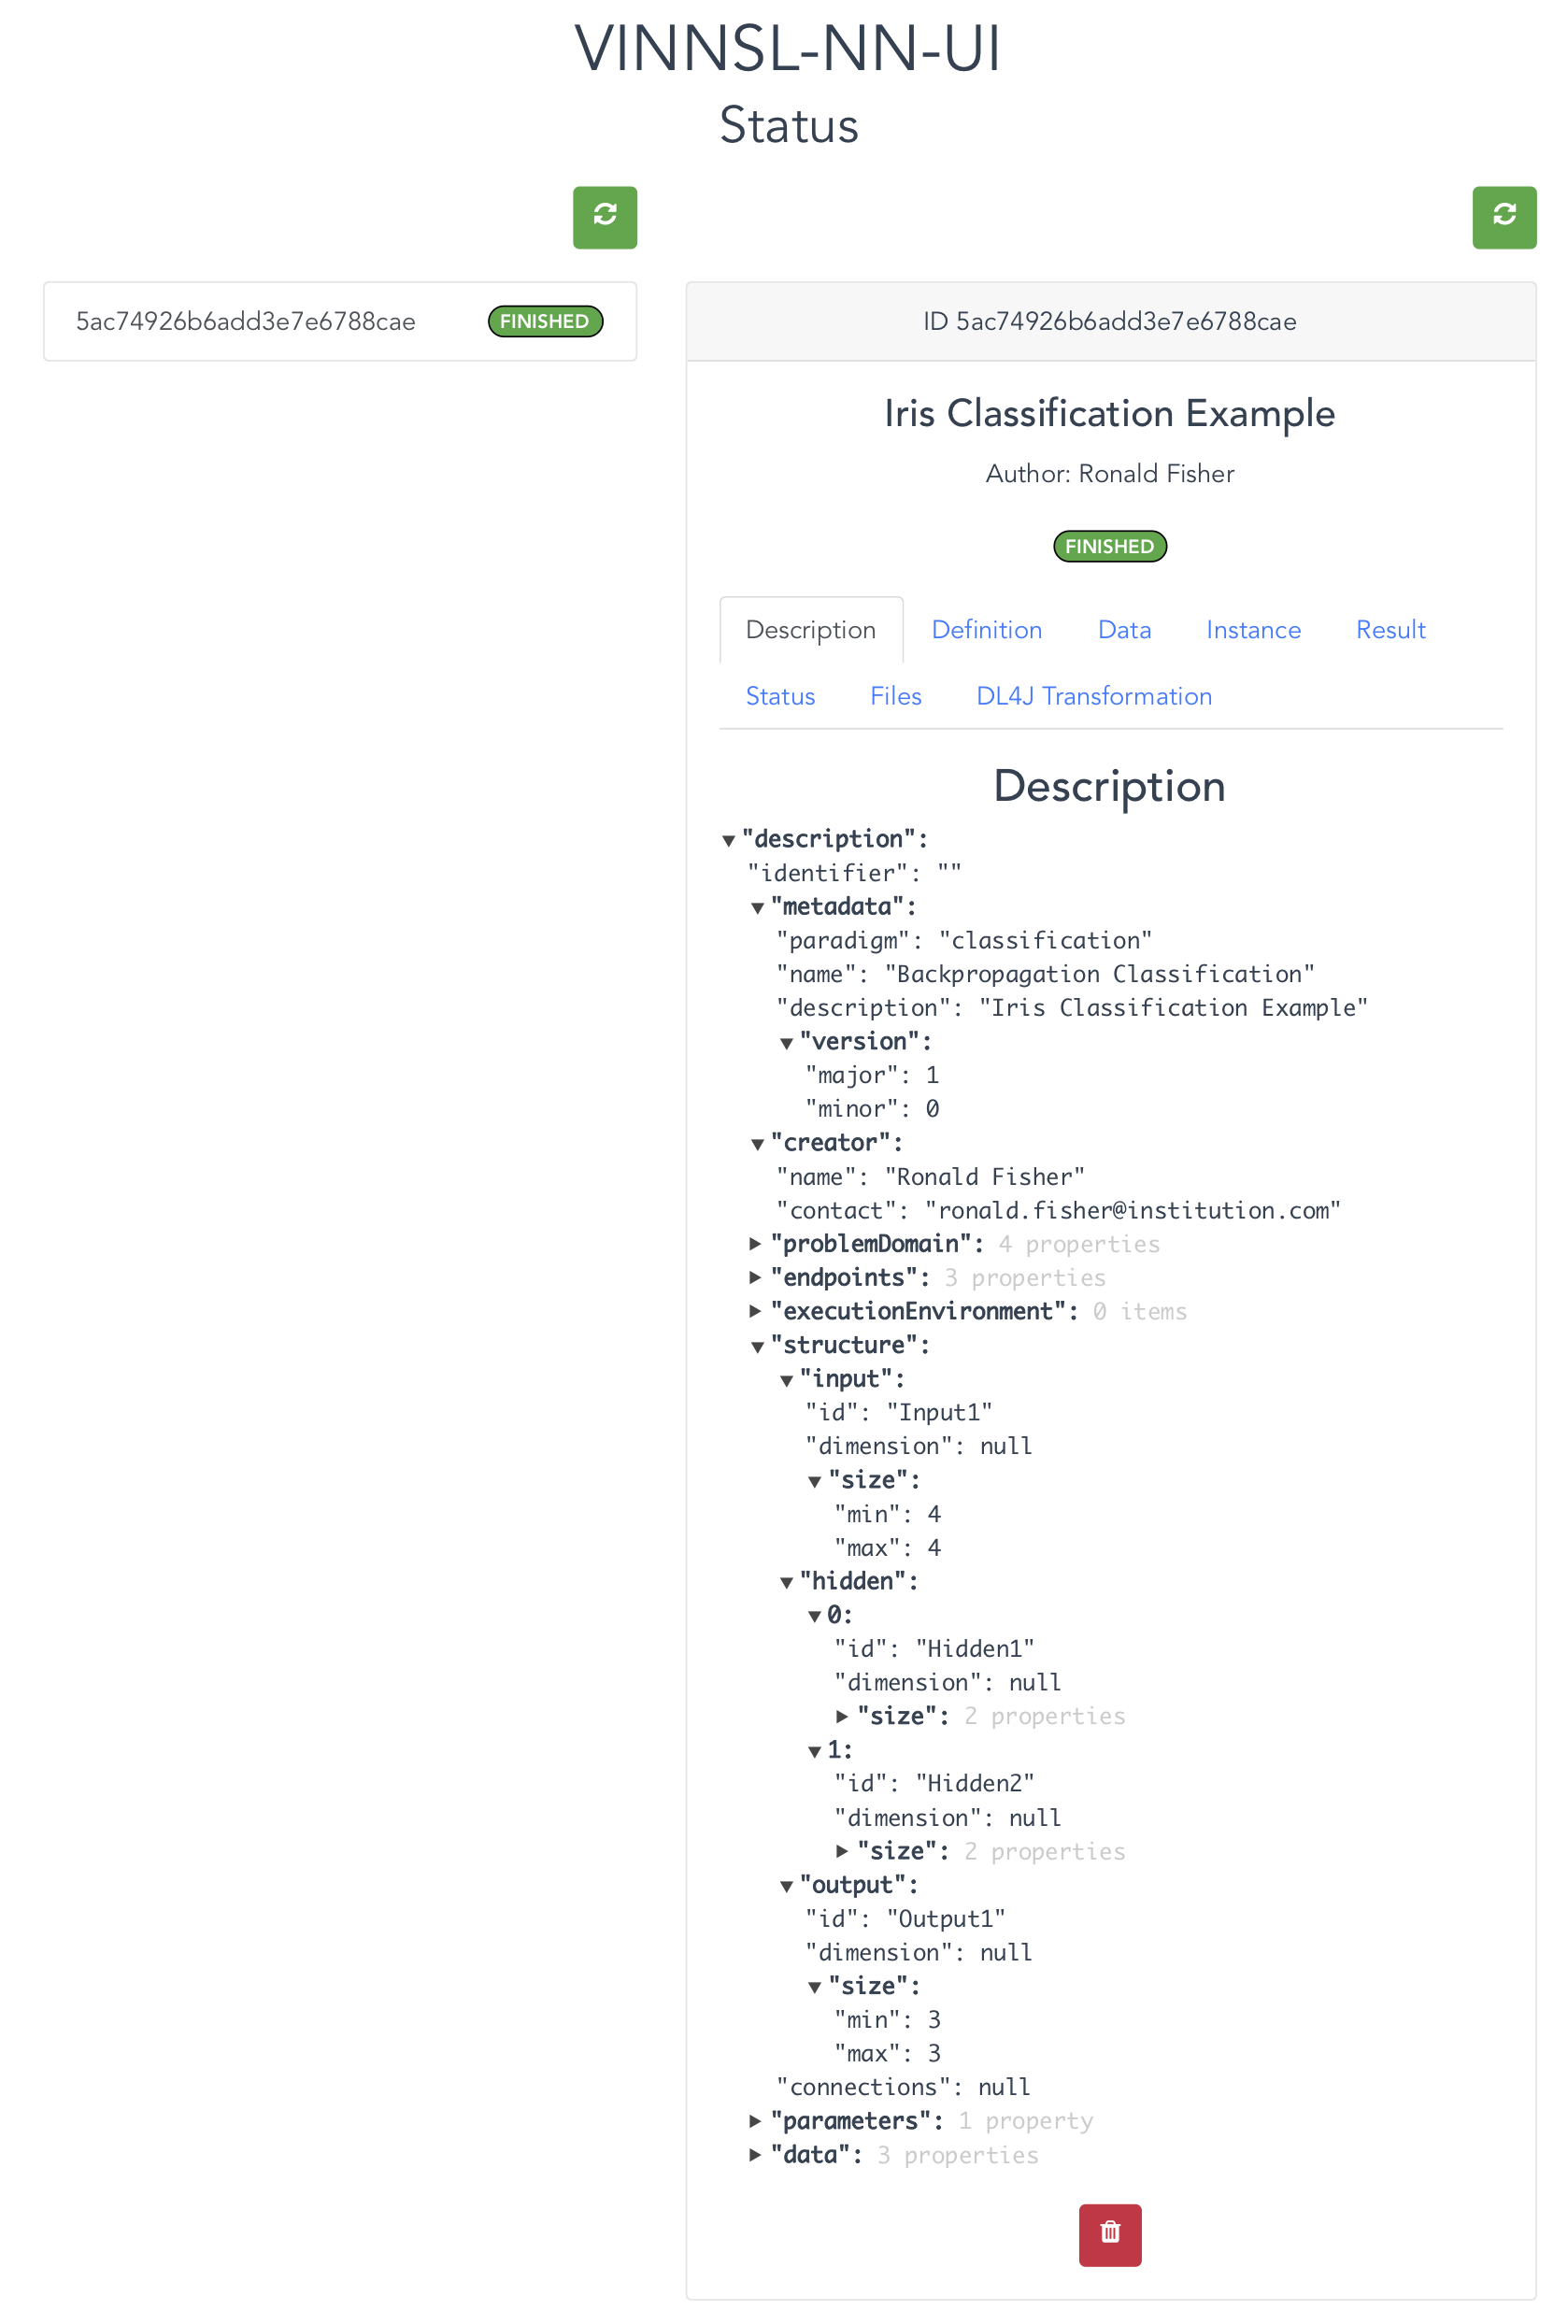
\includegraphics[width=15.00000cm]{images/VINNSL-NN-UI}
\caption{User Interface of Prototype}
\end{figure}

\chapter{Use Cases}\label{use-cases}

\begin{enumerate}
\def\labelenumi{\arabic{enumi})}
\item
  iris classification
\item
  MNIST?
\item
  hosted trained network
\end{enumerate}

\chapter{Future Work}\label{future-work}

TODO

\begin{itemize}
\tightlist
\item
  more function\\
\item
  backend für tensorflow
\item
  grafischer NN designer
\item
  trainierte netzwerke als webservice veröffentlichen
\item
  integration in knime platform
\end{itemize}

\chapter{Conclusions}\label{conclusions}

\chapter{Acknowledgments}\label{acknowledgments}

\chapter{Dedication}\label{dedication}

\chapter{Appendices}\label{appendices}
